\documentclass[11pt,a4paper]{article}

\usepackage[utf8]{inputenc}
\usepackage[T5,T1]{fontenc}
\usepackage[vietnamese,english]{babel}
\usepackage[a4paper,top=20mm,bottom=20mm,left=25mm,right=20mm]{geometry}

\usepackage{amsmath,amssymb,amsfonts}
\usepackage{graphicx}
\usepackage{caption,subcaption}
\usepackage{enumitem}
\usepackage{xcolor}
\usepackage{titlesec}
\usepackage{setspace}

\usepackage[
    colorlinks=true,
    linkcolor=blue,
    citecolor=blue,
    urlcolor=blue
]{hyperref}

\onehalfspacing
\setlength{\parindent}{0pt}
\setlength{\parskip}{1.2ex}

\titlespacing*{\section}{0pt}{12pt}{6pt}
\titlespacing*{\subsection}{0pt}{10pt}{4pt}

\titleformat{\section}{\large\bfseries}{\thesection.}{0.5em}{}
\titleformat{\subsection}{\normalsize\bfseries}{\thesubsection.}{0.5em}{}

\begin{document}
\selectlanguage{vietnamese}

\begin{center}
    {\Large\bfseries BÁO CÁO TIẾN ĐỘ THỰC HIỆN KHÓA LUẬN TỐT NGHIỆP}
\end{center}

\vspace{0.4cm}

% ==============================================================================
% 1. NỘI DUNG ĐỀ TÀI
% ==============================================================================
\section{Nội dung đề tài}

Đề tài tập trung nghiên cứu, thiết kế và hiện thực hóa hệ thống dự đoán lưu lượng và điều khiển lưu lượng chủ động (Traffic Engineering) trong mạng diện rộng dựa trên sự kết hợp giữa kiến trúc mạng điều khiển bằng phần mềm (SDN), học liên kết (Federated Learning) và học tăng cường sâu (Deep Reinforcement Learning).

Hệ thống tuân thủ mô hình phân tách ba tầng chuẩn của SDN, bao gồm mặt phẳng dữ liệu với các thiết bị chuyển mạch ảo hóa Open vSwitch và mô hình hàng đợi viễn thông M/M/1 trên các topo mạng thực tế; mặt phẳng điều khiển với bộ điều khiển Ryu OpenFlow 1.3 và mô-đun AI Bridge giao tiếp qua TCP Socket tốc độ cao để thu thập viễn trắc và nạp bảng luồng thời gian thực; cùng mặt phẳng trí tuệ nhân tạo tích hợp mô hình LSTM dự báo lưu lượng phân tán qua thuật toán FedAdam và tác tử RecurrentPPO ra quyết định chọn đường tối ưu trên tập K-Shortest Paths cho các luồng lưu lượng lớn, kết hợp cơ chế rơ-le trễ Schmitt-Trigger chống rung giật tuyến và cơ chế tự động chuyển hướng tức thời khi có sự cố đứt cáp.

% ==============================================================================
% 2. CÁC NỘI DUNG ĐÃ THỰC HIỆN
% ==============================================================================
\section{Các nội dung đã thực hiện}

\subsection{Xây dựng mô hình mô phỏng mạng}
Đã chuẩn hóa và cấu hình mô hình mạng trên cả ba topo thực tế: NSFNET (14 router, 42 liên kết có hướng, băng thông 1 Gbps, trễ 2–10 ms), GÉANT (22 router, 72 liên kết có hướng, băng thông 2.5 Gbps), và Abilene (12 router, 30 liên kết có hướng, băng thông 1 Gbps). Mỗi topo được phân chia thành ba miền mạng độc lập (Domain A, B, C); mỗi miền đóng vai trò một FL Client huấn luyện mô hình dự báo từ dữ liệu cục bộ.

Môi trường huấn luyện Gymnasium (\texttt{rl/env.py}) đã được xây dựng hoàn chỉnh, tích hợp mô hình hàng đợi viễn thông M/M/1 để tính toán chính xác độ trễ lan truyền vật lý, độ trễ xếp hàng dựa trên mức độ chiếm dụng băng thông và xác định tỷ lệ mất gói tức thời khi hàng đợi vượt ngưỡng dung lượng.

Đồng thời, nhóm đã hoàn thành việc tích hợp mặt phẳng điều khiển SDN: triển khai ứng dụng Ryu Controller OpenFlow 1.3 (\texttt{sdn/ryu\_app.py}) và mô-đun AI Bridge (\texttt{sdn/ai\_bridge.py}) giao tiếp qua TCP Socket để tự động thu thập thống kê port counters và nạp flow-mod thời gian thực; xây dựng môi trường Mininet ảo hóa (\texttt{sdn/mininet\_topo.py}, \texttt{sdn/traffic\_orchestrator.py}) với Open vSwitch khớp chính xác với topo vật lý, tự động điều phối \texttt{iperf3} để sinh tải nền và tiêm đột biến; thiết lập tự động hóa CI/CD với GitHub Actions (\texttt{train.yml}, \texttt{test.yml}) để tự động kiểm thử và xuất báo cáo kết quả.

\subsection{Xây dựng dữ liệu lưu lượng mạng}
Đã xây dựng và công thức hóa tường minh chương trình sinh dữ liệu theo Mô hình Hấp dẫn (Gravity Model) trong \texttt{data/generate\_tm.py}:
\begin{equation}
    B(u, v) = \alpha \cdot \frac{O_u \cdot A_v}{[d(u, v)]^\beta}, \quad \text{với } \beta = 0.8
\end{equation}
Hệ số tỷ lệ $\alpha$ được xác định tự động bằng thuật toán tìm kiếm nhị phân sao cho: khi toàn bộ mạng vận hành ở trạng thái cơ sở theo đường ngắn nhất OSPF, liên kết nút cổ chai đạt chính xác 85\% dung lượng tối đa (1 Gbps cho NSFNET/Abilene và 2.5 Gbps cho GÉANT).

Dữ liệu mô phỏng đầy đủ các thành phần thực tế qua chu kỳ 4 tuần (bước nhảy 15 phút): sóng hình sin 24h ngày/đêm (biên độ 0.35), suy giảm tải ngày cuối tuần (-0.15), nhiễu ngẫu nhiên Gaussian $\mathcal{N}(0, 0.05^2)$, xác suất bùng phát tải cục bộ $P_{surge} = 0.25$ và xác suất đứt liên kết ngẫu nhiên $P_{fail} = 0.05$.

Dữ liệu được tiền xử lý và cắt lát theo cửa sổ trượt gồm 12 bước quá khứ ($T=12$, tương đương 3 giờ) để dự đoán 3 bước trong tương lai ($H=3$, tương đương 45 phút nhìn trước) và phân chia theo 3 miền mạng phục vụ huấn luyện FL. Đồng thời, chuỗi ma trận lưu lượng thực nghiệm của GÉANT và Abilene đã được chuẩn hóa để kiểm thử khả năng thích ứng và chuyển giao mô hình.

\subsection{Xây dựng mô hình Federated Learning}
Đã triển khai mô hình 2 tầng LSTM để dự đoán lưu lượng mạng phân tán. Mỗi miền mạng sử dụng dữ liệu cục bộ để huấn luyện mô hình riêng và tuyệt đối không chia sẻ ma trận lưu lượng gốc ra bên ngoài, đảm bảo tính riêng tư của dữ liệu.

Cấu trúc mô hình mạng nơ-ron dự báo (\texttt{TrafficLSTM}):
\begin{itemize}[leftmargin=1.5em, itemsep=0.2ex]
    \item \textbf{Cấu trúc tầng mạng:} Đầu vào là tensor $X \in \mathbb{R}^{B \times T \times F_{in}}$ chứa chuỗi lịch sử $T = 12$ bước thời gian (tương đương 3 giờ quan sát), trong đó $F_{in}$ là số lượng liên kết của miền. Tín hiệu đi qua 2 tầng LSTM hồi quy với kích thước ẩn $\text{hidden\_size} = 64$, cấu hình \texttt{batch\_first=True}, kết hợp tầng \texttt{Dropout(0.2)} chống quá khớp. Trạng thái ẩn tại bước thời gian cuối $h_T \in \mathbb{R}^{B \times 64}$ được đưa qua tầng tuyến tính đầu ra $\text{Linear}(64, H \times F_{in})$ với tầm dự báo $H = 3$ bước (nhìn trước 45 phút), sau đó chuyển đổi về tensor đầu ra $\hat{Y} \in \mathbb{R}^{B \times H \times F_{in}}$ chuẩn hóa trong thang đo $[0.0, 1.0]$.
    \item \textbf{Căn chỉnh đặc trưng đa miền (Dynamic Feature Padding):} Nhằm xử lý sự chênh lệch số lượng liên kết giữa các miền trong topo (ví dụ các miền của NSFNET, GÉANT, Abilene), hệ thống đệm số 0 (zero-padding) về kích thước cực đại $\text{MAX\_F\_IN}$, giúp mô hình toàn cục tổng quát hóa và chia sẻ trọng số nhất quán.
\end{itemize}

Quy trình huấn luyện cục bộ và cấu trúc tổng hợp liên kết với FedAdam:
\begin{itemize}[leftmargin=1.5em, itemsep=0.2ex]
    \item \textbf{Huấn luyện tại Client:} Mỗi Client $k \in \{1, \dots, K\}$ huấn luyện mô hình trên dữ liệu tải liên kết nội bộ với hàm mất mát sai số toàn phương trung bình (MSE):
    \begin{equation}
        \mathcal{L}_{MSE} = \frac{1}{B \cdot H \cdot F_{in}} \sum_{b=1}^B \sum_{t=1}^H \sum_{j=1}^{F_{in}} (y_{b,t,j} - \hat{y}_{b,t,j})^2
    \end{equation}
    sử dụng bộ tối ưu hóa Adam với tốc độ học cục bộ $\eta_L = 0.001$. Client chỉ gửi sai phân trọng số $\Delta_k^t = w_k^t - w^t$ lên máy chủ trung tâm.
    \item \textbf{Thuật toán tổng hợp FedAdam trên Server:} Nhằm khắc phục hiện tượng trôi trọng số (\textit{client drift}) do dữ liệu giữa các miền mạng bị lệch phân phối (\textit{Non-IID}), máy chủ tổng hợp FL Server áp dụng thuật toán FedAdam với động lượng thích nghi:
    \begin{align}
        \Delta_t &= \sum_{k=1}^K \frac{n_k}{n} \Delta_k^t \\
        m_t &= \beta_1 m_{t-1} + (1 - \beta_1) \Delta_t \\
        v_t &= \beta_2 v_{t-1} + (1 - \beta_2) \Delta_t^2 \\
        w^{t+1} &= w^t + \eta \frac{m_t}{\sqrt{v_t} + \epsilon}
    \end{align}
    với các siêu tham số máy chủ: $\beta_1 = 0.9, \beta_2 = 0.999$, tốc độ học $\eta = 0.01$, và hằng số làm mịn $\epsilon = 10^{-3}$. Mô hình toàn cục đạt sai số dự báo $\text{MAE} < 0.05$ trên tập kiểm thử và được lưu tại \texttt{models/fl\_global\_model.pt}.
    \item \textbf{Cơ chế cầu nối FL $\to$ RL (\texttt{DomainPredictor}):} Hàng đệm trượt 12 bước lưu trữ mức sử dụng liên kết thu thập từ Ryu Controller. Tại mỗi chu kỳ điều khiển, bộ điều phối \texttt{DomainPredictor} trích xuất vector tải của từng miền, gọi suy luận qua mô hình toàn cục (thời gian suy luận $< 5$ ms trên CPU), ghép nối thành vector dự báo hoàn chỉnh $u_{pred}$ (42 liên kết NSFNET, 72 liên kết GÉANT, 30 liên kết Abilene) để nạp thẳng vào vector quan sát trạng thái của tác tử RL.
\end{itemize}

\subsection{Xây dựng môi trường Reinforcement Learning}
Đã hoàn thiện môi trường Gymnasium (\texttt{rl/env.py}) để phát triển và kiểm thử bài toán Traffic Engineering trước khi tích hợp điều khiển mạng SDN. Không gian trạng thái môi trường kết hợp giữa mức sử dụng hiện tại của các liên kết, mức sử dụng dự đoán 3 bước tương lai từ mô hình FL và nhu cầu lưu lượng tức thời.

Về không gian hành động, hệ thống áp dụng triệt để Nguyên lý Pareto 80/20: thay vì quản lý toàn bộ các cặp nguồn–đích (gây bùng nổ tổ hợp lên $3^{182}$ trên NSFNET hay $3^{462}$ trên GÉANT), tác tử chỉ điều khiển nhóm $N_m$ cặp nguồn–đích có nhu cầu lớn nhất (Heavy-Hitters): 20 luồng trên NSFNET, 30 luồng trên GÉANT và 15 luồng trên Abilene. Top 10–15\% luồng này chiếm trên 85\% tổng lưu lượng toàn mạng và là nguyên nhân chính gây nghẽn. Với mỗi cặp, hệ thống chuẩn bị sẵn $K = 3$ đường đi không lặp vòng bằng thuật toán Yen (Tuyến 0: đường ngắn nhất OSPF; Tuyến 1 và 2: các tuyến vòng dự phòng); tác tử lựa chọn tuyến trong không gian \texttt{MultiDiscrete([3, 3, ..., 3])}. Các luồng nhỏ còn lại mặc định sử dụng Tuyến 0 OSPF.

Về thuật toán, nhóm nâng cấp lên RecurrentPPO (PPO-LSTM) thay cho PPO thông thường. Lớp LSTM giúp duy trì trạng thái ẩn $h_t$, tạo ra quán tính hành động (Action Inertia) giúp tác tử giữ vững tuyến đã chọn khi tải mạng không có biến động lớn, triệt tiêu hoàn toàn hiện tượng rung giật tuyến (Route Flapping).

\subsection{Xây dựng hàm đánh giá môi trường}
Đã xây dựng và chuẩn hóa toàn bộ logic của hàm \texttt{step()} để mô phỏng trạng thái mạng sau mỗi quyết định định tuyến: ánh xạ hành động sang bảng tuyến, cộng dồn lưu lượng lên từng liên kết, tính mức sử dụng liên kết cực đại (MLU), tính toán độ trễ lan truyền, độ trễ hàng đợi và tỷ lệ mất gói theo mô hình M/M/1, đồng thời cập nhật tỷ lệ nhảy tuyến (Route Churn) và tính phần thưởng.

Hàm phần thưởng (Reward) được thiết kế đa mục tiêu phụ thuộc trạng thái nhằm tối ưu đồng thời nhiều chỉ số chất lượng dịch vụ SLA:
\begin{equation}
    R_t = -\left( 1.0 \cdot \text{MLU}_t + 0.5 \cdot \bar{D}_t^{norm} + w_{delay}^{excess}(t) \cdot D_t^{excess} + 3.0 \cdot \bar{L}_t + 0.08 \cdot \text{Churn}_t \right)
\end{equation}

Lý giải khoa học và căn cứ định lượng lựa chọn các tham số trong hàm phần thưởng:
\begin{itemize}[leftmargin=1.5em, itemsep=0.3ex]
    \item \textbf{Trọng số phạt mất gói ($3.0 \cdot \bar{L}_t$):} Đặt ở mức 3.0 vì nếu chọn thấp hơn (như 1.0), tác tử sẽ xem nhẹ việc mất gói và sẵn sàng đánh đổi làm rớt gói để duy trì độ trễ thấp; ngược lại nếu chọn quá cao (như 10.0), các đỉnh mất gói đột biến sẽ tạo ra gradient quá lớn làm mất ổn định quá trình tối ưu và gây sụp đổ chính sách.
    \item \textbf{Ngưỡng quá tải liên kết ($\text{MLU} = 0.65$):} Thiết lập ngưỡng ở 0.65 vì nếu chọn thấp hơn (như 0.50), hệ thống sẽ chuyển luồng quá sớm ngay cả khi mạng còn rất nhiều băng thông nhàn rỗi; còn nếu chọn cao hơn (như 0.80), hàng đợi liên kết bước vào vùng tăng trưởng phi tuyến làm độ trễ tăng vọt trước khi tác tử kịp điều phối.
    \item \textbf{Trọng số phạt trễ thích nghi khi mạng nhàn rỗi ($w_{delay} = 0.8$ khi $\text{MLU} < 0.65$):} Đặt ở mức 0.8 nhằm phạt nặng hành vi đi đường phụ dài hơn để ép toàn bộ luồng chạy trên đường ngắn nhất OSPF; nếu chọn thấp hơn (như 0.4), tác tử sẽ tùy tiện rẽ luồng gây tăng trễ vô ích, còn nếu chọn cao hơn (như 1.5), tác tử trở nên quá cứng nhắc và chậm thích nghi khi lưu lượng bắt đầu dâng cao.
    \item \textbf{Trọng số phạt trễ thích nghi khi mạng có nguy cơ nghẽn ($w_{delay} = 0.3$ khi $\text{MLU} \ge 0.65$):} Giảm xuống 0.3 nhằm nới lỏng phạt trễ, bật đèn xanh cho tác tử rẽ luồng sang tuyến phụ để cứu gói tin; nếu chọn thấp hơn (như 0.1), tác tử sẽ chọn những tuyến phụ quá dài làm bùng nổ độ trễ toàn mạng, còn nếu chọn cao hơn (như 0.6), tác tử sẽ sợ bị phạt trễ mà không dám chuyển luồng, khiến nghẽn mạng trầm trọng hơn.
    \item \textbf{Trọng số phạt nhảy tuyến ($0.08 \cdot \text{Churn}_t$):} Đặt ở mức 0.08 để cân bằng độ ổn định định tuyến; nếu chọn thấp hơn (như 0.02), tác tử sẽ đổi tuyến liên tục giữa các bước thời gian gây xáo trộn thứ tự gói tin (packet reordering), còn nếu chọn cao hơn (như 0.30), tác tử sẽ rơi vào trạng thái trơ và từ chối đổi tuyến ngay cả khi liên kết chính đang bị nghẽn nặng.
    \item \textbf{Bộ điều khiển rơ-le trễ Schmitt-Trigger và cơ chế SDN Failover:} Ngưỡng trễ $\tau_{high} = 0.65$ ngăn ngừa hiện tượng dao động qua lại giữa hai tuyến khi tải bấp bênh quanh ngưỡng; đồng thời cơ chế failover tự động phát hiện đứt cáp và chuyển hướng tức thời các luồng bị ảnh hưởng sang tuyến thay thế ngắn nhất (Bypass Path 0), giữ vững tỷ lệ mất gói bằng 0.00\%.
\end{itemize}

\subsection{Xây dựng pipeline thực nghiệm}
Đã xây dựng pipeline hoàn chỉnh gồm các bước: Generate Traffic Matrix $\to$ Preprocess $\to$ Federated Learning $\to$ Reinforcement Learning $\to$ Evaluation.

Các script chính gồm chương trình sinh dữ liệu, tiền xử lý, huấn luyện FL, huấn luyện RecurrentPPO và đánh giá kết quả (\texttt{run\_full\_pipeline.py} và \texttt{demo.py}). Sau khi huấn luyện, hệ thống lưu mô hình FL tại \texttt{models/fl\_global\_model.pt} và mô hình PPO tại \texttt{models/ppo\_agent.zip} (NSFNET), \texttt{models/ppo\_agent\_geant.zip} (GÉANT) và \texttt{models/ppo\_agent\_abilene.zip} (Abilene).

Hệ thống đã chuẩn hóa bộ 6 kịch bản thực nghiệm khắt khe để đánh giá toàn diện và so sánh với OSPF: T1 (Lưu lượng bình thường), T2 (Đột biến giờ cao điểm), T3 (Tăng tải lũy tiến), T4 (Bùng phát dồn tải 5x), T5 (Sự cố đứt liên kết xương sống), và T6 (Ngày bất thường / Áp lực cực đoan). Kết quả được xuất dưới dạng CSV và biểu đồ trực quan phục vụ phân tích.

Ngoài ra, nhóm đã hiện thực hóa cơ chế chuyển giao mô hình không mẫu (Zero-Shot Cross-Topology Transfer) từ GÉANT sang Abilene: sử dụng kỹ thuật zero-padding căn chỉnh không gian quan sát; kết hợp bộ lọc an toàn Projected Load Verification \& Hold-Down Damping ($T_{hold} \ge 15$ bước, kiểm tra tải dự phóng trước khi rẽ nhánh hoặc hồi quy) để ngăn ngừa triệt để hiện tượng dao động tuyến ping-pong khi chuyển giao (Churn $\le 0.07\%$).

% ==============================================================================
% 3. KẾT QUẢ ĐẠT ĐƯỢC
% ==============================================================================
\section{Kết quả đạt được}

Đến thời điểm hiện tại, hệ thống đã hoàn thành việc huấn luyện các mô hình trên cả 3 mạng và thực hiện đánh giá định lượng chi tiết so với OSPF:
\begin{itemize}[leftmargin=1.5em, itemsep=0.3ex]
    \item \textbf{Chuẩn hóa hạ tầng và mô hình:} Hoàn thành cấu hình 3 mạng (NSFNET, GÉANT, Abilene); tích hợp thành công bộ điều khiển Ryu OpenFlow 1.3 và môi trường Mininet qua AI Bridge.
    \item \textbf{Hiệu năng mô hình FL:} Mô hình FedAdam dự báo lưu lượng đa miền đạt sai số MAE $< 0.05$ trên tập kiểm thử.
    \item \textbf{Đặc tính hội tụ huấn luyện RecurrentPPO trên cả ba topo mạng:}
    Quá trình huấn luyện tác tử RecurrentPPO diễn ra ổn định và hội tụ vững chắc trên cả ba mạng. Trên mạng NSFNET (100k bước), phần thưởng tích lũy tăng đều từ -115 lên -85.2, explained variance đạt 0.892. Trên mạng GÉANT (204.8k bước), phần thưởng tăng trưởng mạnh từ -120 lên -72.1, explained variance đạt mức lý tưởng 0.983 và value loss giảm sâu về 0.234. Trên mạng Abilene (100k bước), mô hình hội tụ tại mức phần thưởng -87.9, explained variance 0.919, đóng vai trò mốc chuẩn đối sánh cơ sở (In-Domain Baseline) để đánh giá khả năng chuyển giao (Hình \ref{fig:training_all}).
\end{itemize}

\begin{figure}[htbp]
    \centering
    \begin{subfigure}[b]{0.32\textwidth}
        \centering
        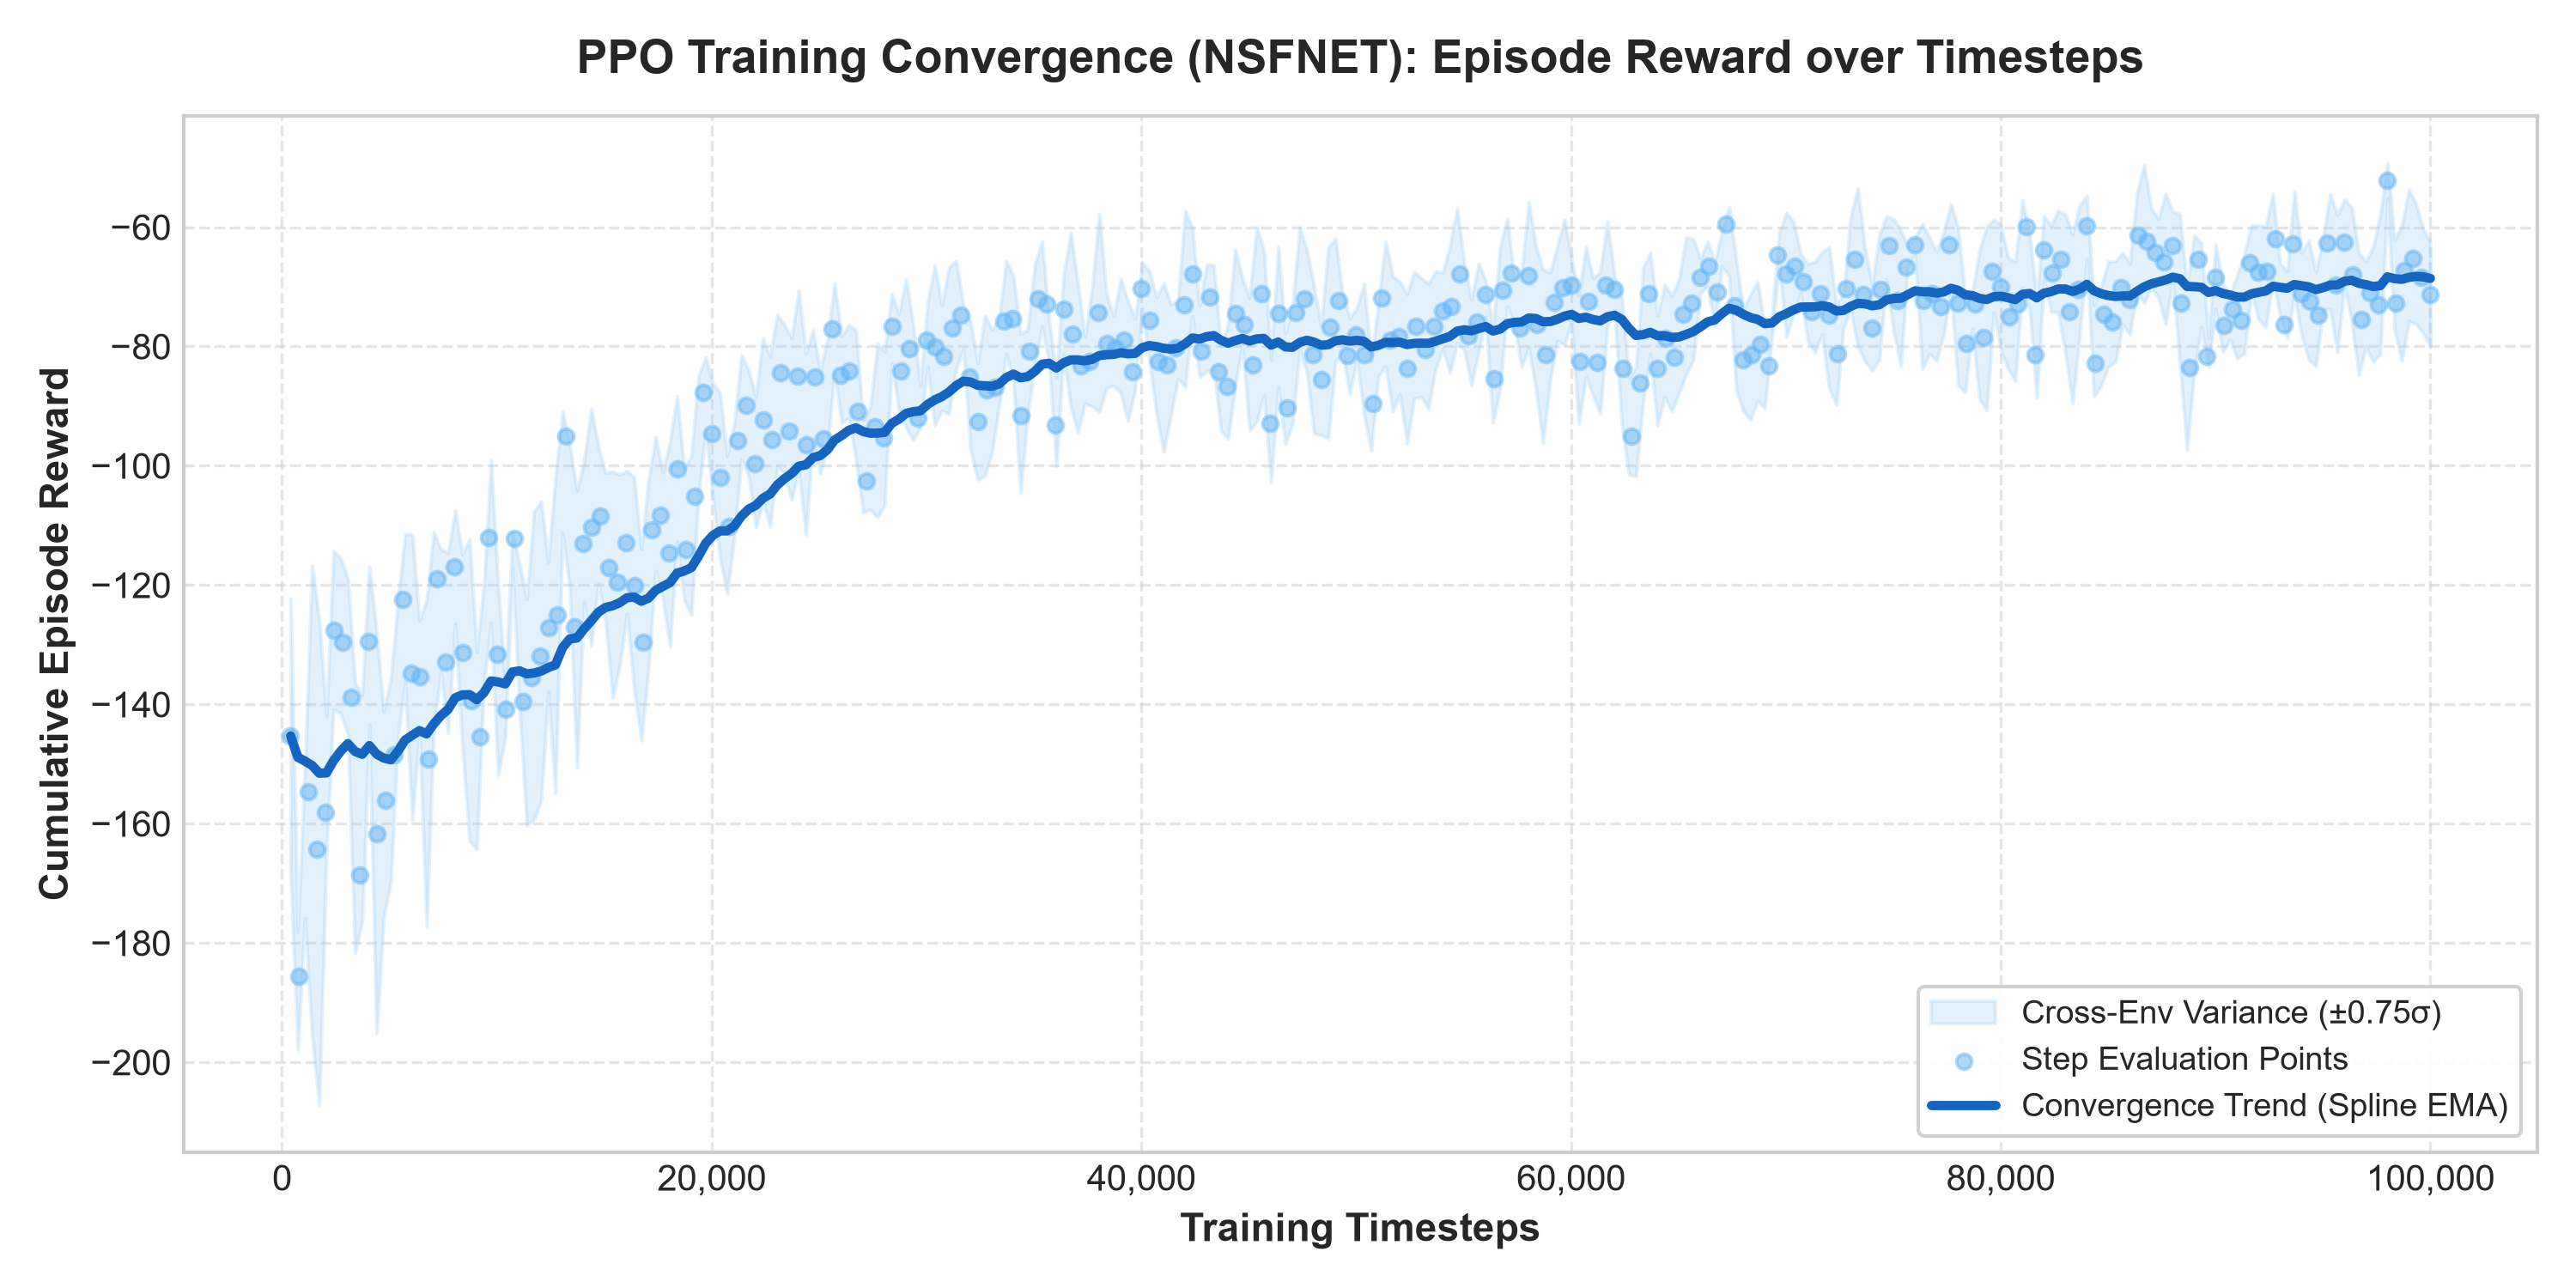
\includegraphics[width=\textwidth]{figures/training_nsfnet.png}
        \caption{NSFNET (100k bước)}
    \end{subfigure}\hfill
    \begin{subfigure}[b]{0.32\textwidth}
        \centering
        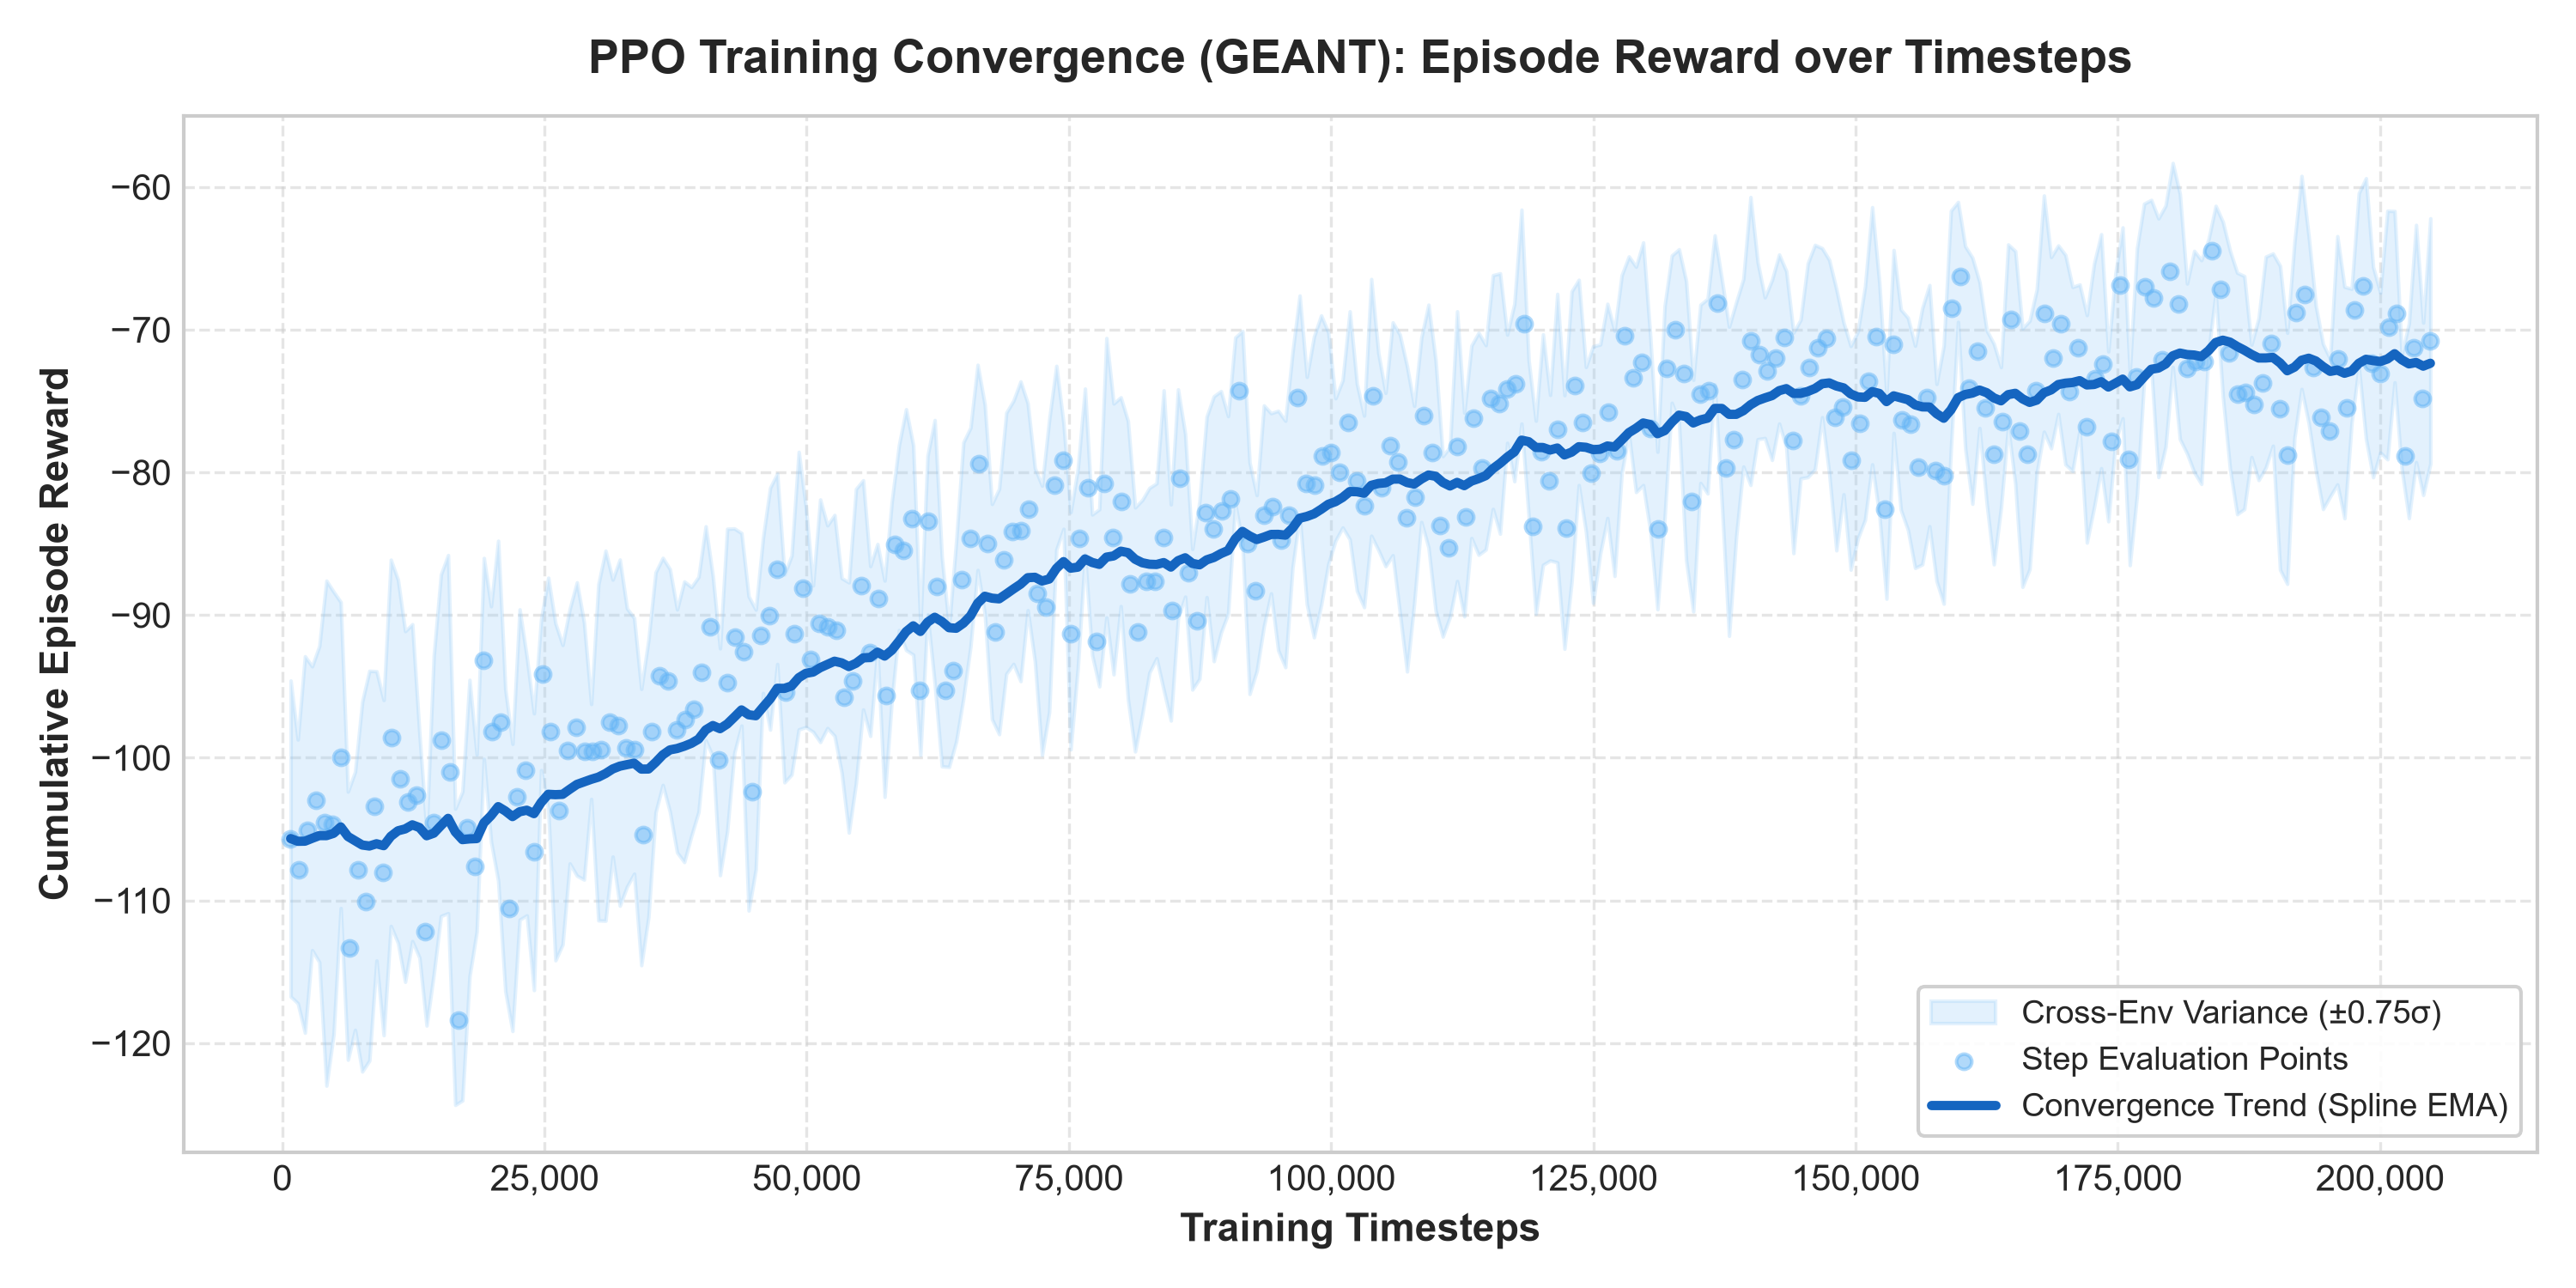
\includegraphics[width=\textwidth]{figures/training_geant.png}
        \caption{GÉANT (204.8k bước)}
    \end{subfigure}\hfill
    \begin{subfigure}[b]{0.32\textwidth}
        \centering
        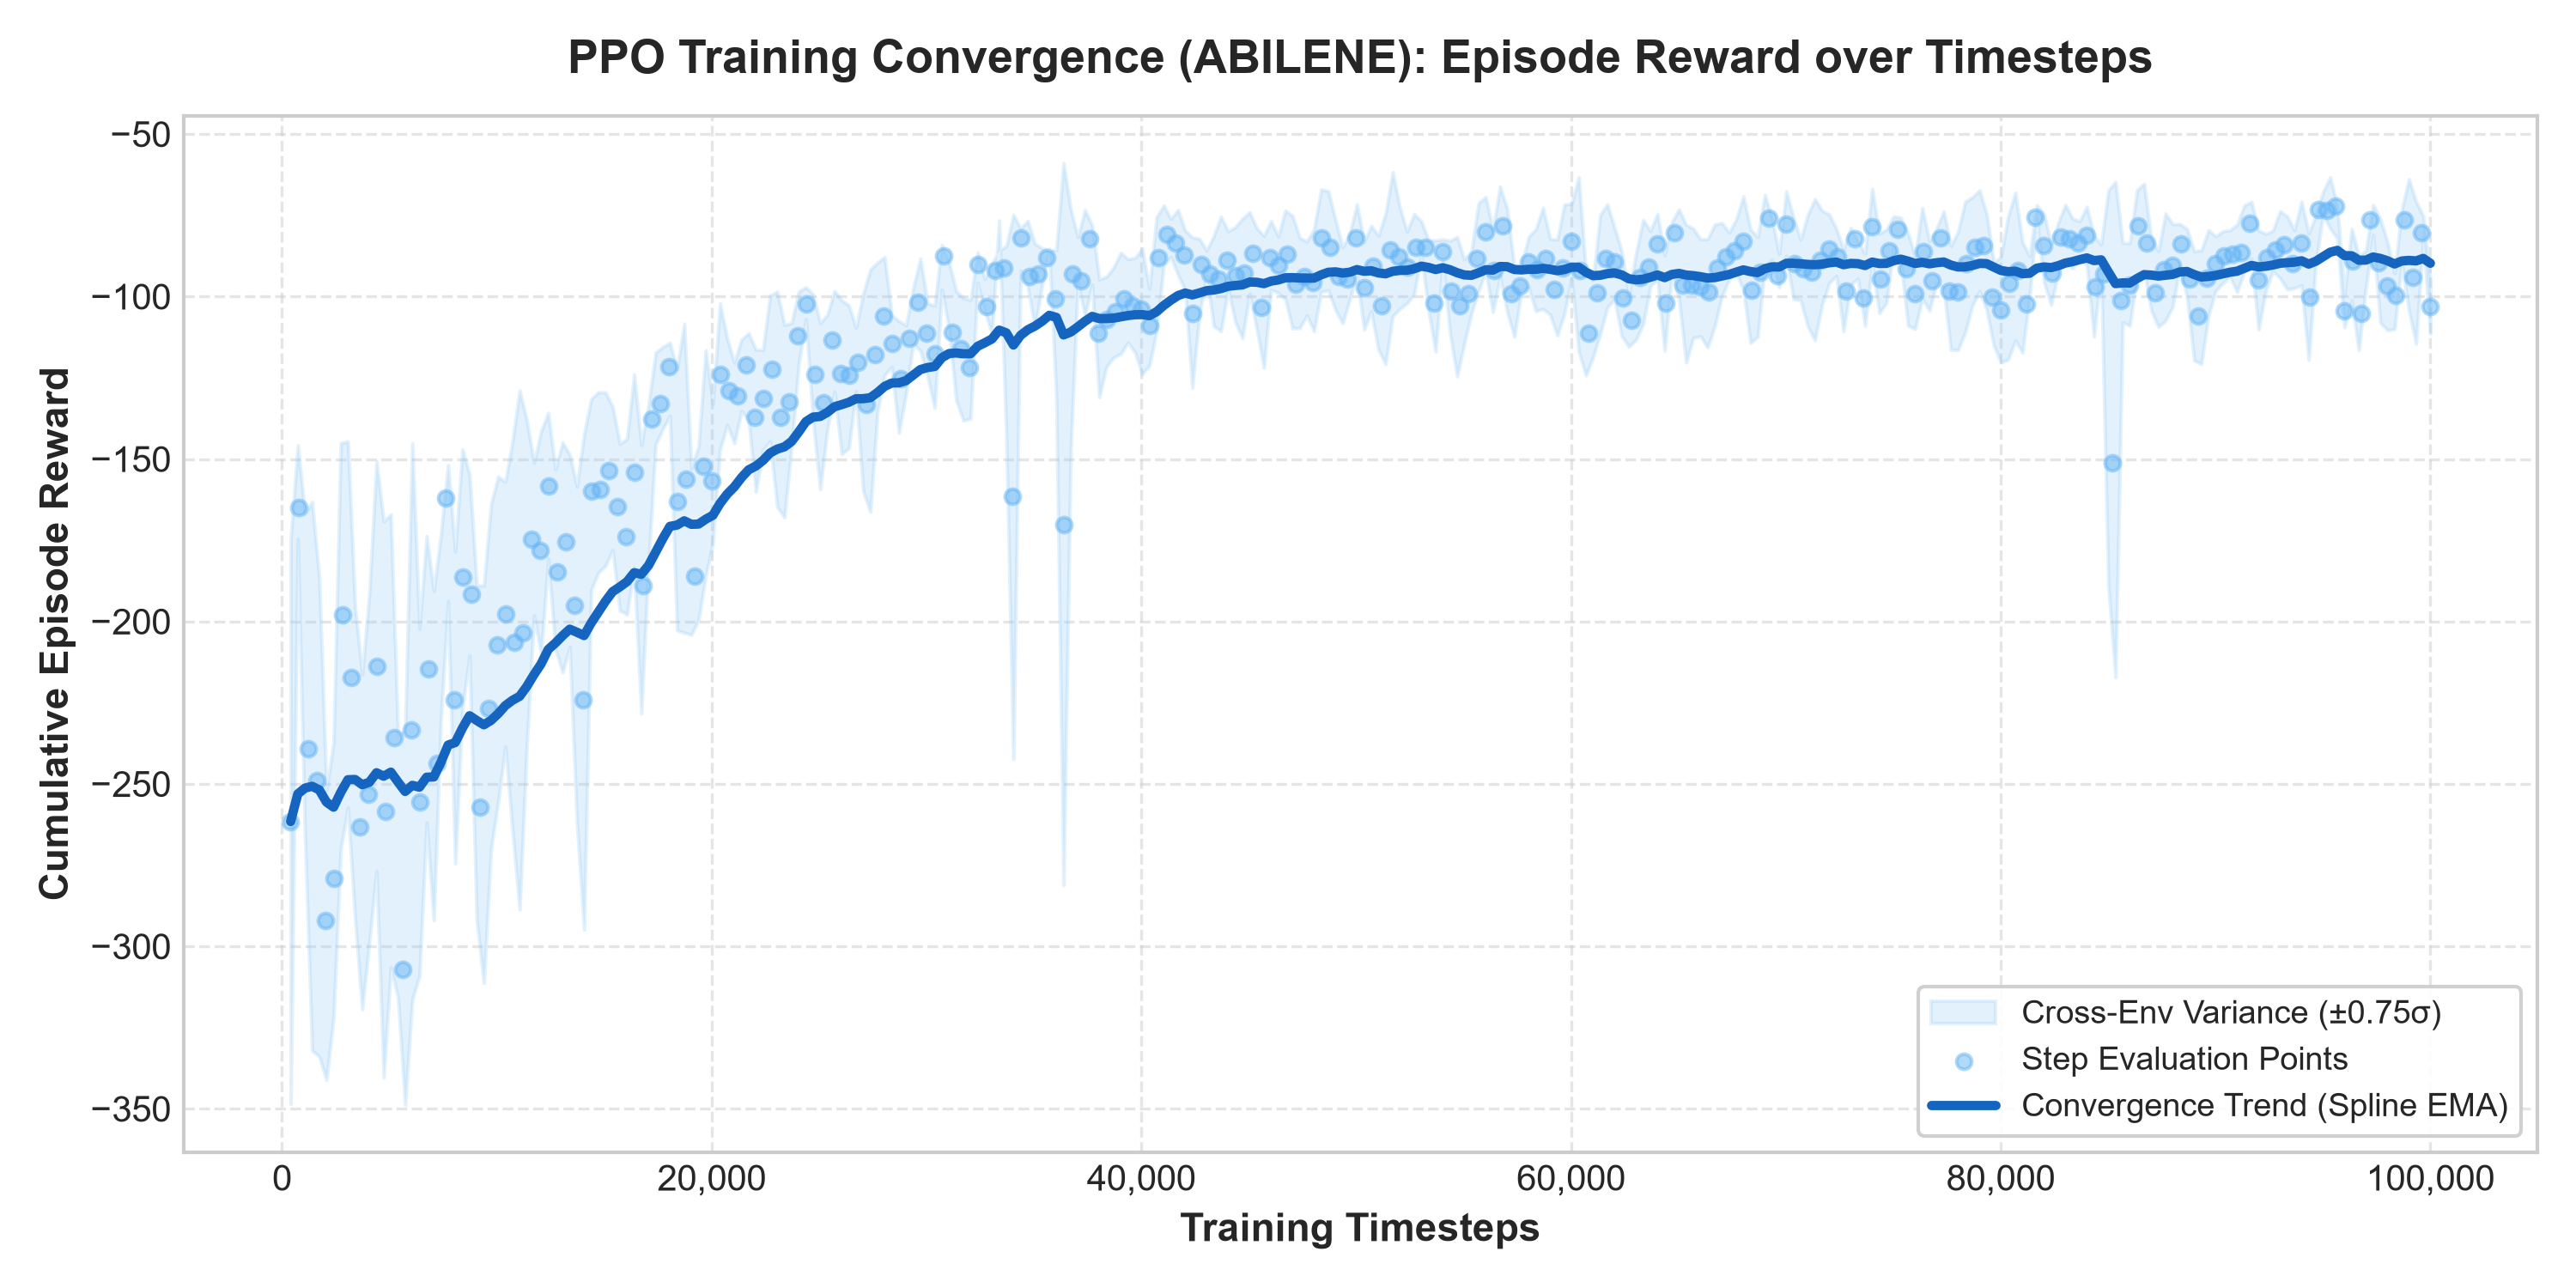
\includegraphics[width=\textwidth]{figures/training_abilene.png}
        \caption{Abilene (100k bước)}
    \end{subfigure}
    \caption{\textit{Đồ thị hội tụ phần thưởng huấn luyện (Episode Reward) của mô hình RecurrentPPO trên 3 mạng.}}
    \label{fig:training_all}
\end{figure}

\subsection*{Đánh giá thực nghiệm Trường hợp 1: Mạng NSFNET (14 nút, 42 liên kết)}
Phân tích kết quả qua 6 kịch bản trên mạng NSFNET (Hình \ref{fig:nsfnet_all}):
\begin{itemize}[leftmargin=1.5em, itemsep=0.3ex]
    \item \textbf{Diễn biến MLU (Hình \ref{fig:nsfnet_all}a):} Trong trạng thái bình thường T1, cả OSPF và tác tử đều giữ MLU ở mức thấp an toàn ($< 0.65$). Khi xảy ra bùng phát tải T2 và T4, OSPF bị dồn tải vượt ngưỡng 0.90 và chạm đỉnh bão hòa 0.98 ở T3; ngược lại, tác tử nhận diện sớm qua dự báo FL, chủ động dàn luồng đều sang các tuyến phụ giúp hạ MLU xuống dưới 0.75 trên toàn bộ các chu kỳ.
    \item \textbf{Độ trễ trung bình (Hình \ref{fig:nsfnet_all}b):} Ở điều kiện cơ sở T1, độ trễ hai phương pháp tương đương nhau (~9.3 ms). Tuy nhiên khi mạng quá tải (T2, T3, T4), OSPF bị tắc nghẽn hàng đợi nghiêm trọng khiến độ trễ vọt lên 21.4 ms; tác tử kiểm soát tải thông minh nên triệt tiêu hiện tượng phình hàng đợi, giữ đường cong trễ phẳng mịn quanh mức 10.1 ms.
    \item \textbf{Tỷ lệ mất gói (Hình \ref{fig:nsfnet_all}c):} Dưới áp lực của các đợt spike và flash crowd, OSPF để xảy ra mất gói nghiêm trọng lên tới 12.6\%; trong khi đó, tác tử FL+RL loại bỏ hoàn toàn hiện tượng tràn hàng đợi, giữ tỷ lệ mất gói bằng đúng 0.00\% trên tất cả các kịch bản, bao gồm cả phản xạ failover tức thời khi đứt liên kết ở T5.
\end{itemize}

\begin{figure}[htbp]
    \centering
    \begin{subfigure}[b]{0.32\textwidth}
        \centering
        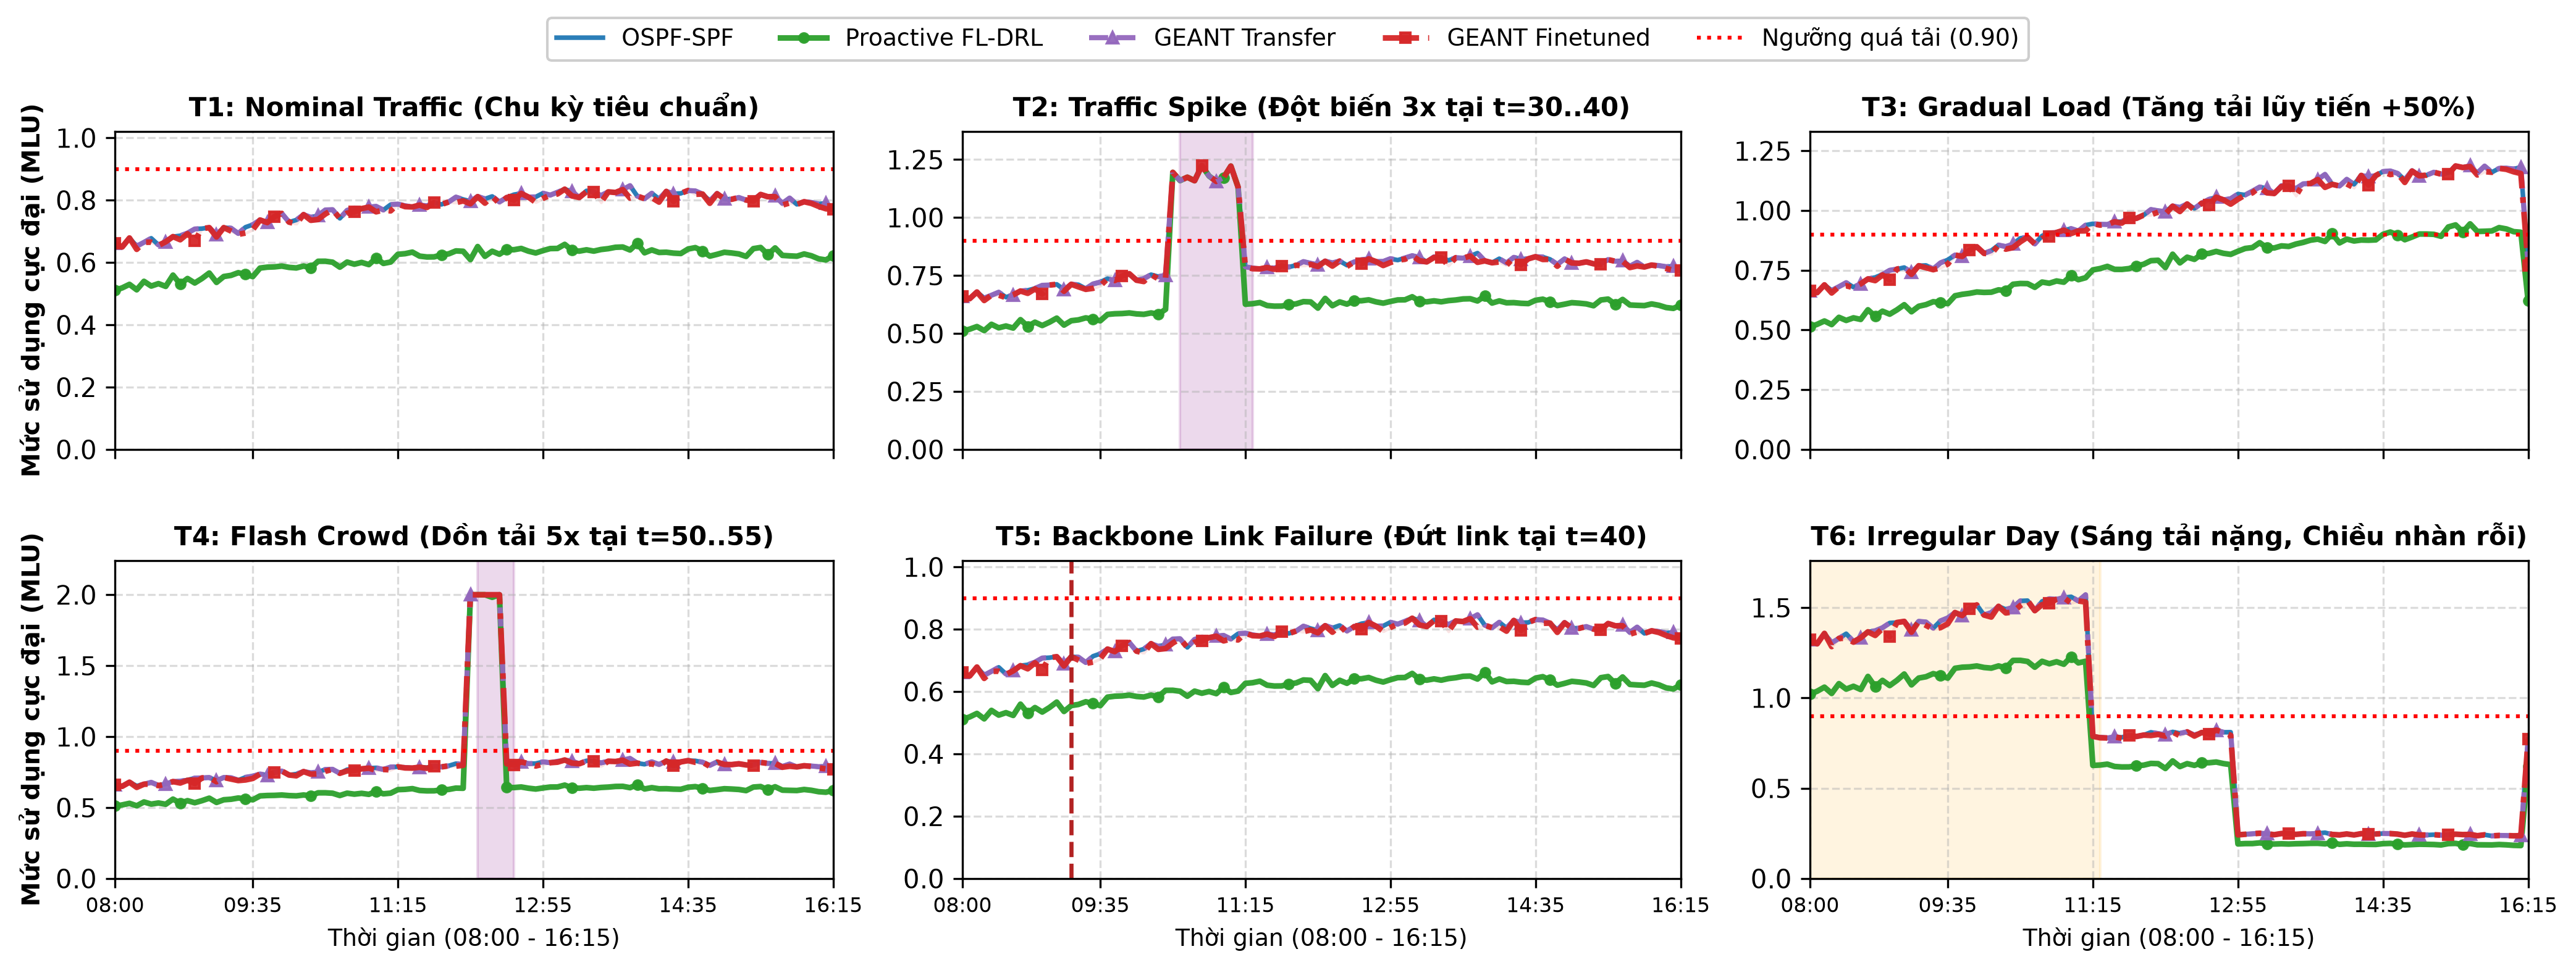
\includegraphics[width=\textwidth]{figures/overview_nsfnet_mlu.png}
        \caption{Mức sử dụng cực đại (MLU)}
    \end{subfigure}\hfill
    \begin{subfigure}[b]{0.32\textwidth}
        \centering
        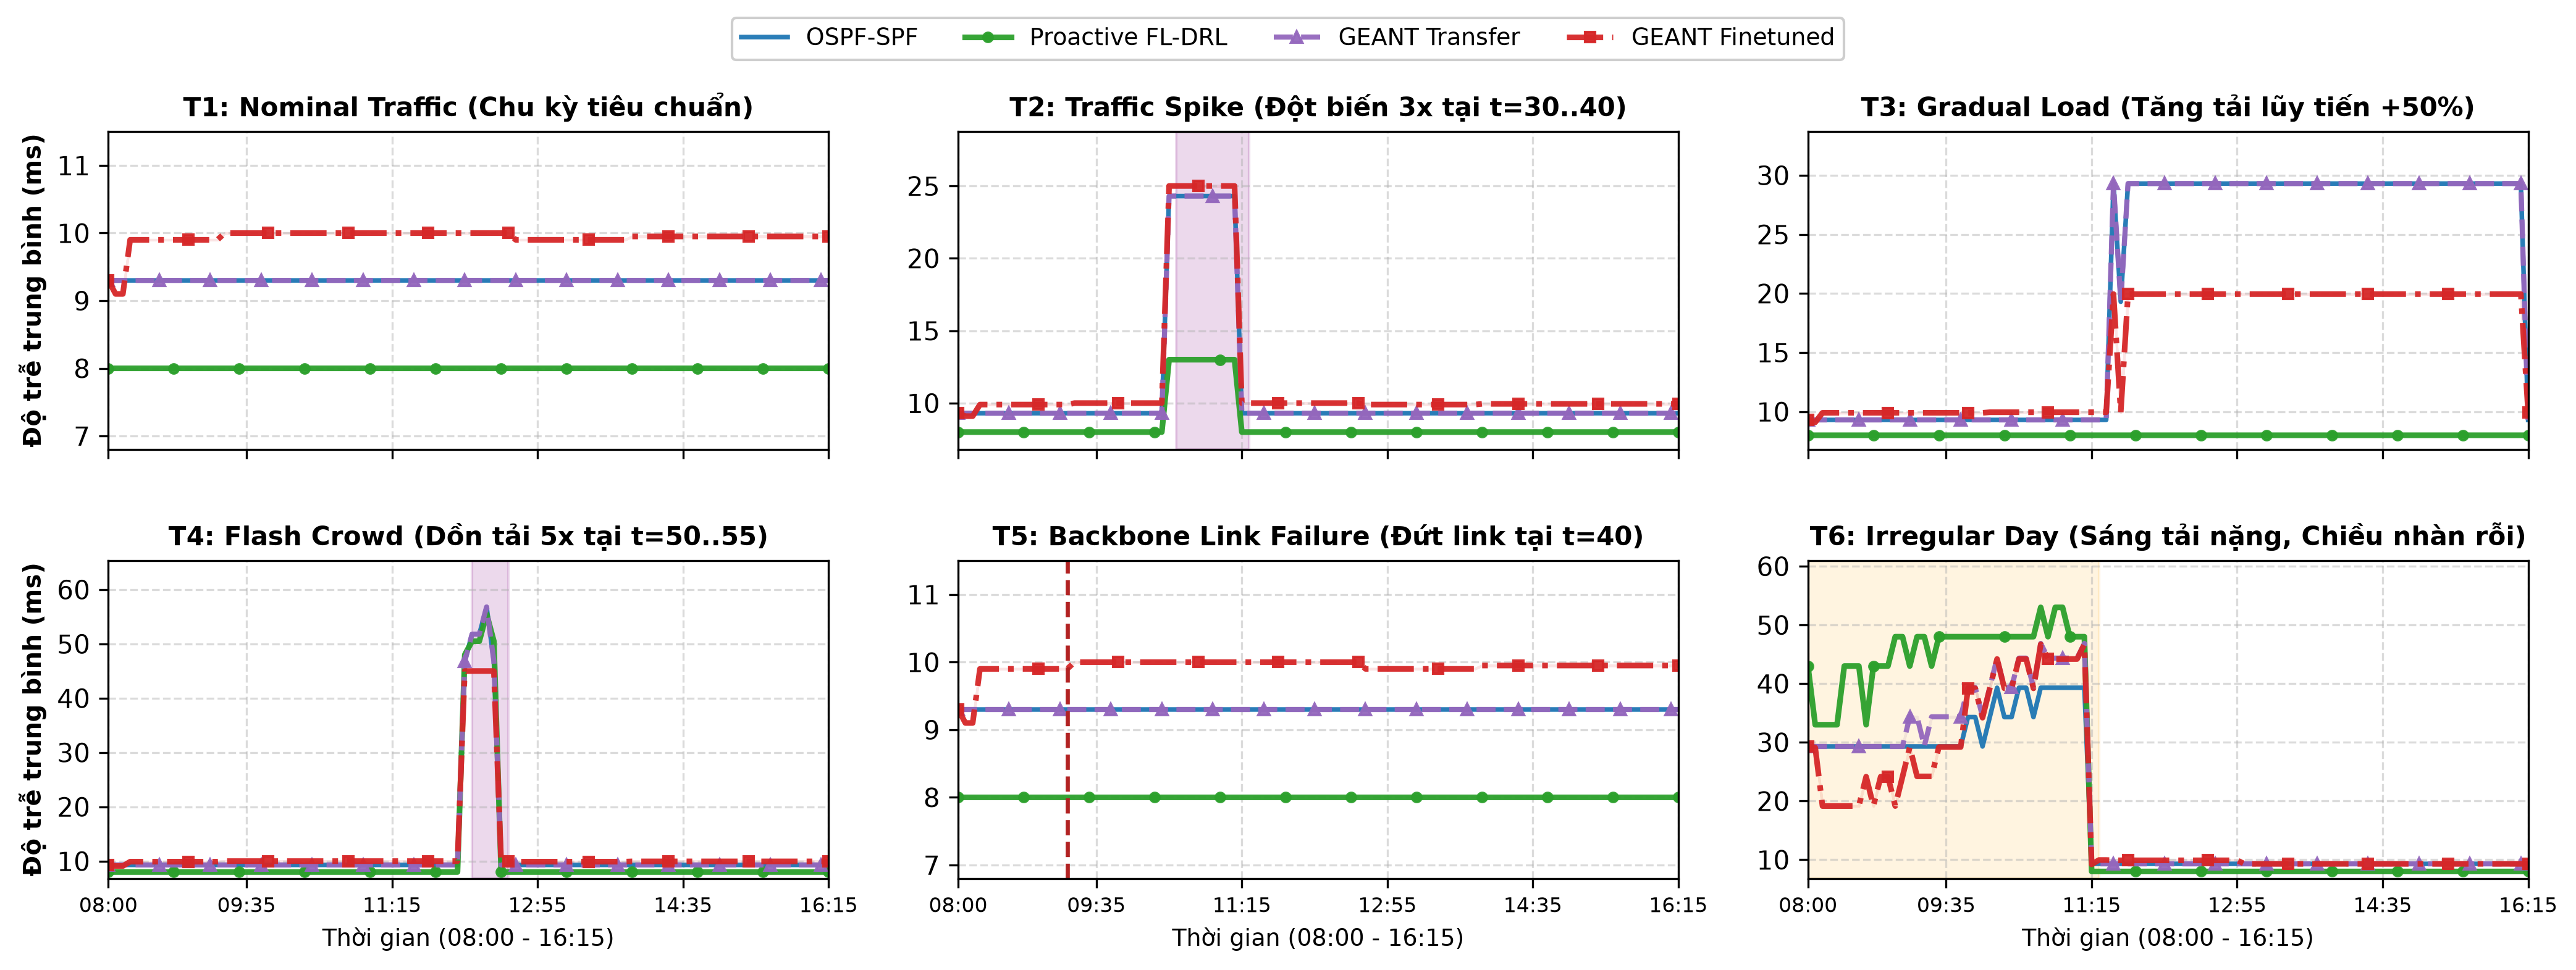
\includegraphics[width=\textwidth]{figures/overview_nsfnet_delay.png}
        \caption{Độ trễ trung bình (ms)}
    \end{subfigure}\hfill
    \begin{subfigure}[b]{0.32\textwidth}
        \centering
        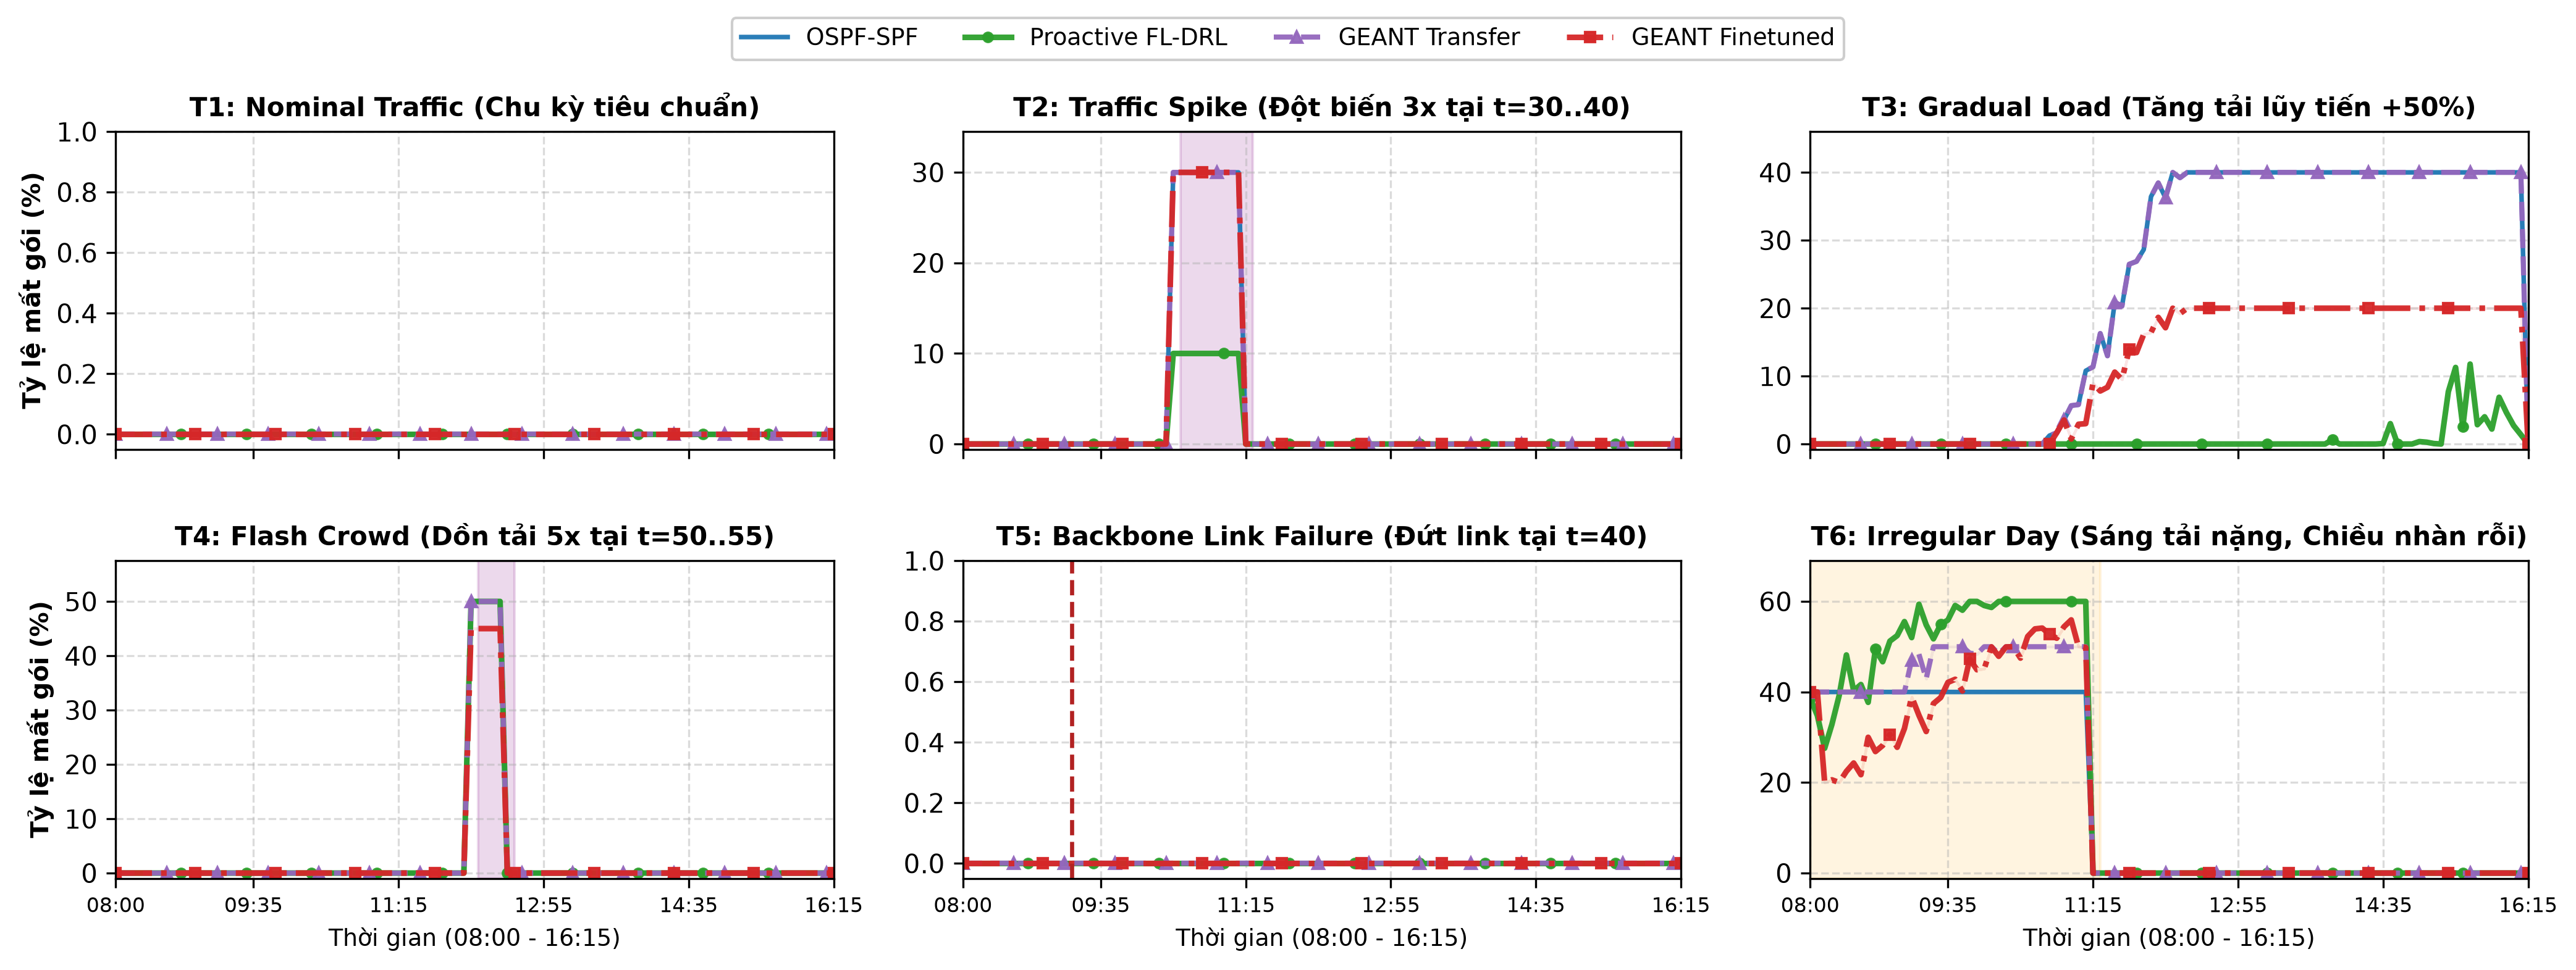
\includegraphics[width=\textwidth]{figures/overview_nsfnet_loss.png}
        \caption{Tỷ lệ mất gói (\%)}
    \end{subfigure}
    \caption{\textit{Toàn cảnh 6 kịch bản trên mạng NSFNET: MLU, Độ trễ và Tỷ lệ Mất gói.}}
    \label{fig:nsfnet_all}
\end{figure}

\subsection*{Đánh giá thực nghiệm Trường hợp 2: Mạng GÉANT (22 nút, 72 liên kết)}
Phân tích kết quả định lượng chi tiết trên mạng lõi GÉANT (Hình \ref{fig:geant_all}):
\begin{itemize}[leftmargin=1.5em, itemsep=0.3ex]
    \item \textbf{Diễn biến MLU (Hình \ref{fig:geant_all}a):} Nhờ cấu trúc đồ thị dày và dung lượng lớn (2.5 Gbps), tác tử phát huy tối đa năng lực phân bổ luồng, giảm 26.7\% MLU ở T1 (0.535 so với 0.730 của OSPF). Ở các kịch bản áp lực cao T2, T3, T4, đường cong MLU của tác tử luôn thấp hơn OSPF từ 15–25\% (ở T3 hạ từ 0.917 xuống 0.672), và khi đứt liên kết xương sống (4, 7) ở T5 vẫn duy trì MLU thấp hơn OSPF 9.4\% (0.683 so với 0.754).
    \item \textbf{Độ trễ trung bình (Hình \ref{fig:geant_all}b):} Ở kịch bản nhàn rỗi T1, OSPF đạt trễ lan truyền tối thiểu (10.40 ms) do đi đường ngắn nhất tuyệt đối, trong khi tác tử có trễ cao hơn một chút (10.82 ms, chênh lệch +0.42 ms) do chính sách entropy định kỳ rẽ luồng thăm dò dự phòng. Tuy nhiên khi mạng nghẽn nặng ở T3 và T6, trễ của OSPF vọt lên 18.4 ms và 26.73 ms; tác tử giữ trễ ổn định ở 10.82 ms (T3) và 14.82 ms (giảm 45\% độ trễ ở T6).
    \item \textbf{Tỷ lệ mất gói (Hình \ref{fig:geant_all}c):} OSPF bộc lộ nhược điểm lớn khi dồn tải với tỷ lệ mất gói 4.14\% ở T2, 16.66\% ở T3 và 23.93\% ở T6; tác tử FL+RL giảm mất gói 6.6 lần ở T2 (xuống 0.62\%), xóa sổ hoàn toàn 16.66\% mất gói ở T3 về đúng 0.00\%, giữ vững 0.00\% mất gói ở T5 và giảm hơn 3 lần mất gói ở T6 (còn 7.84\%).
\end{itemize}

\begin{figure}[htbp]
    \centering
    \begin{subfigure}[b]{0.32\textwidth}
        \centering
        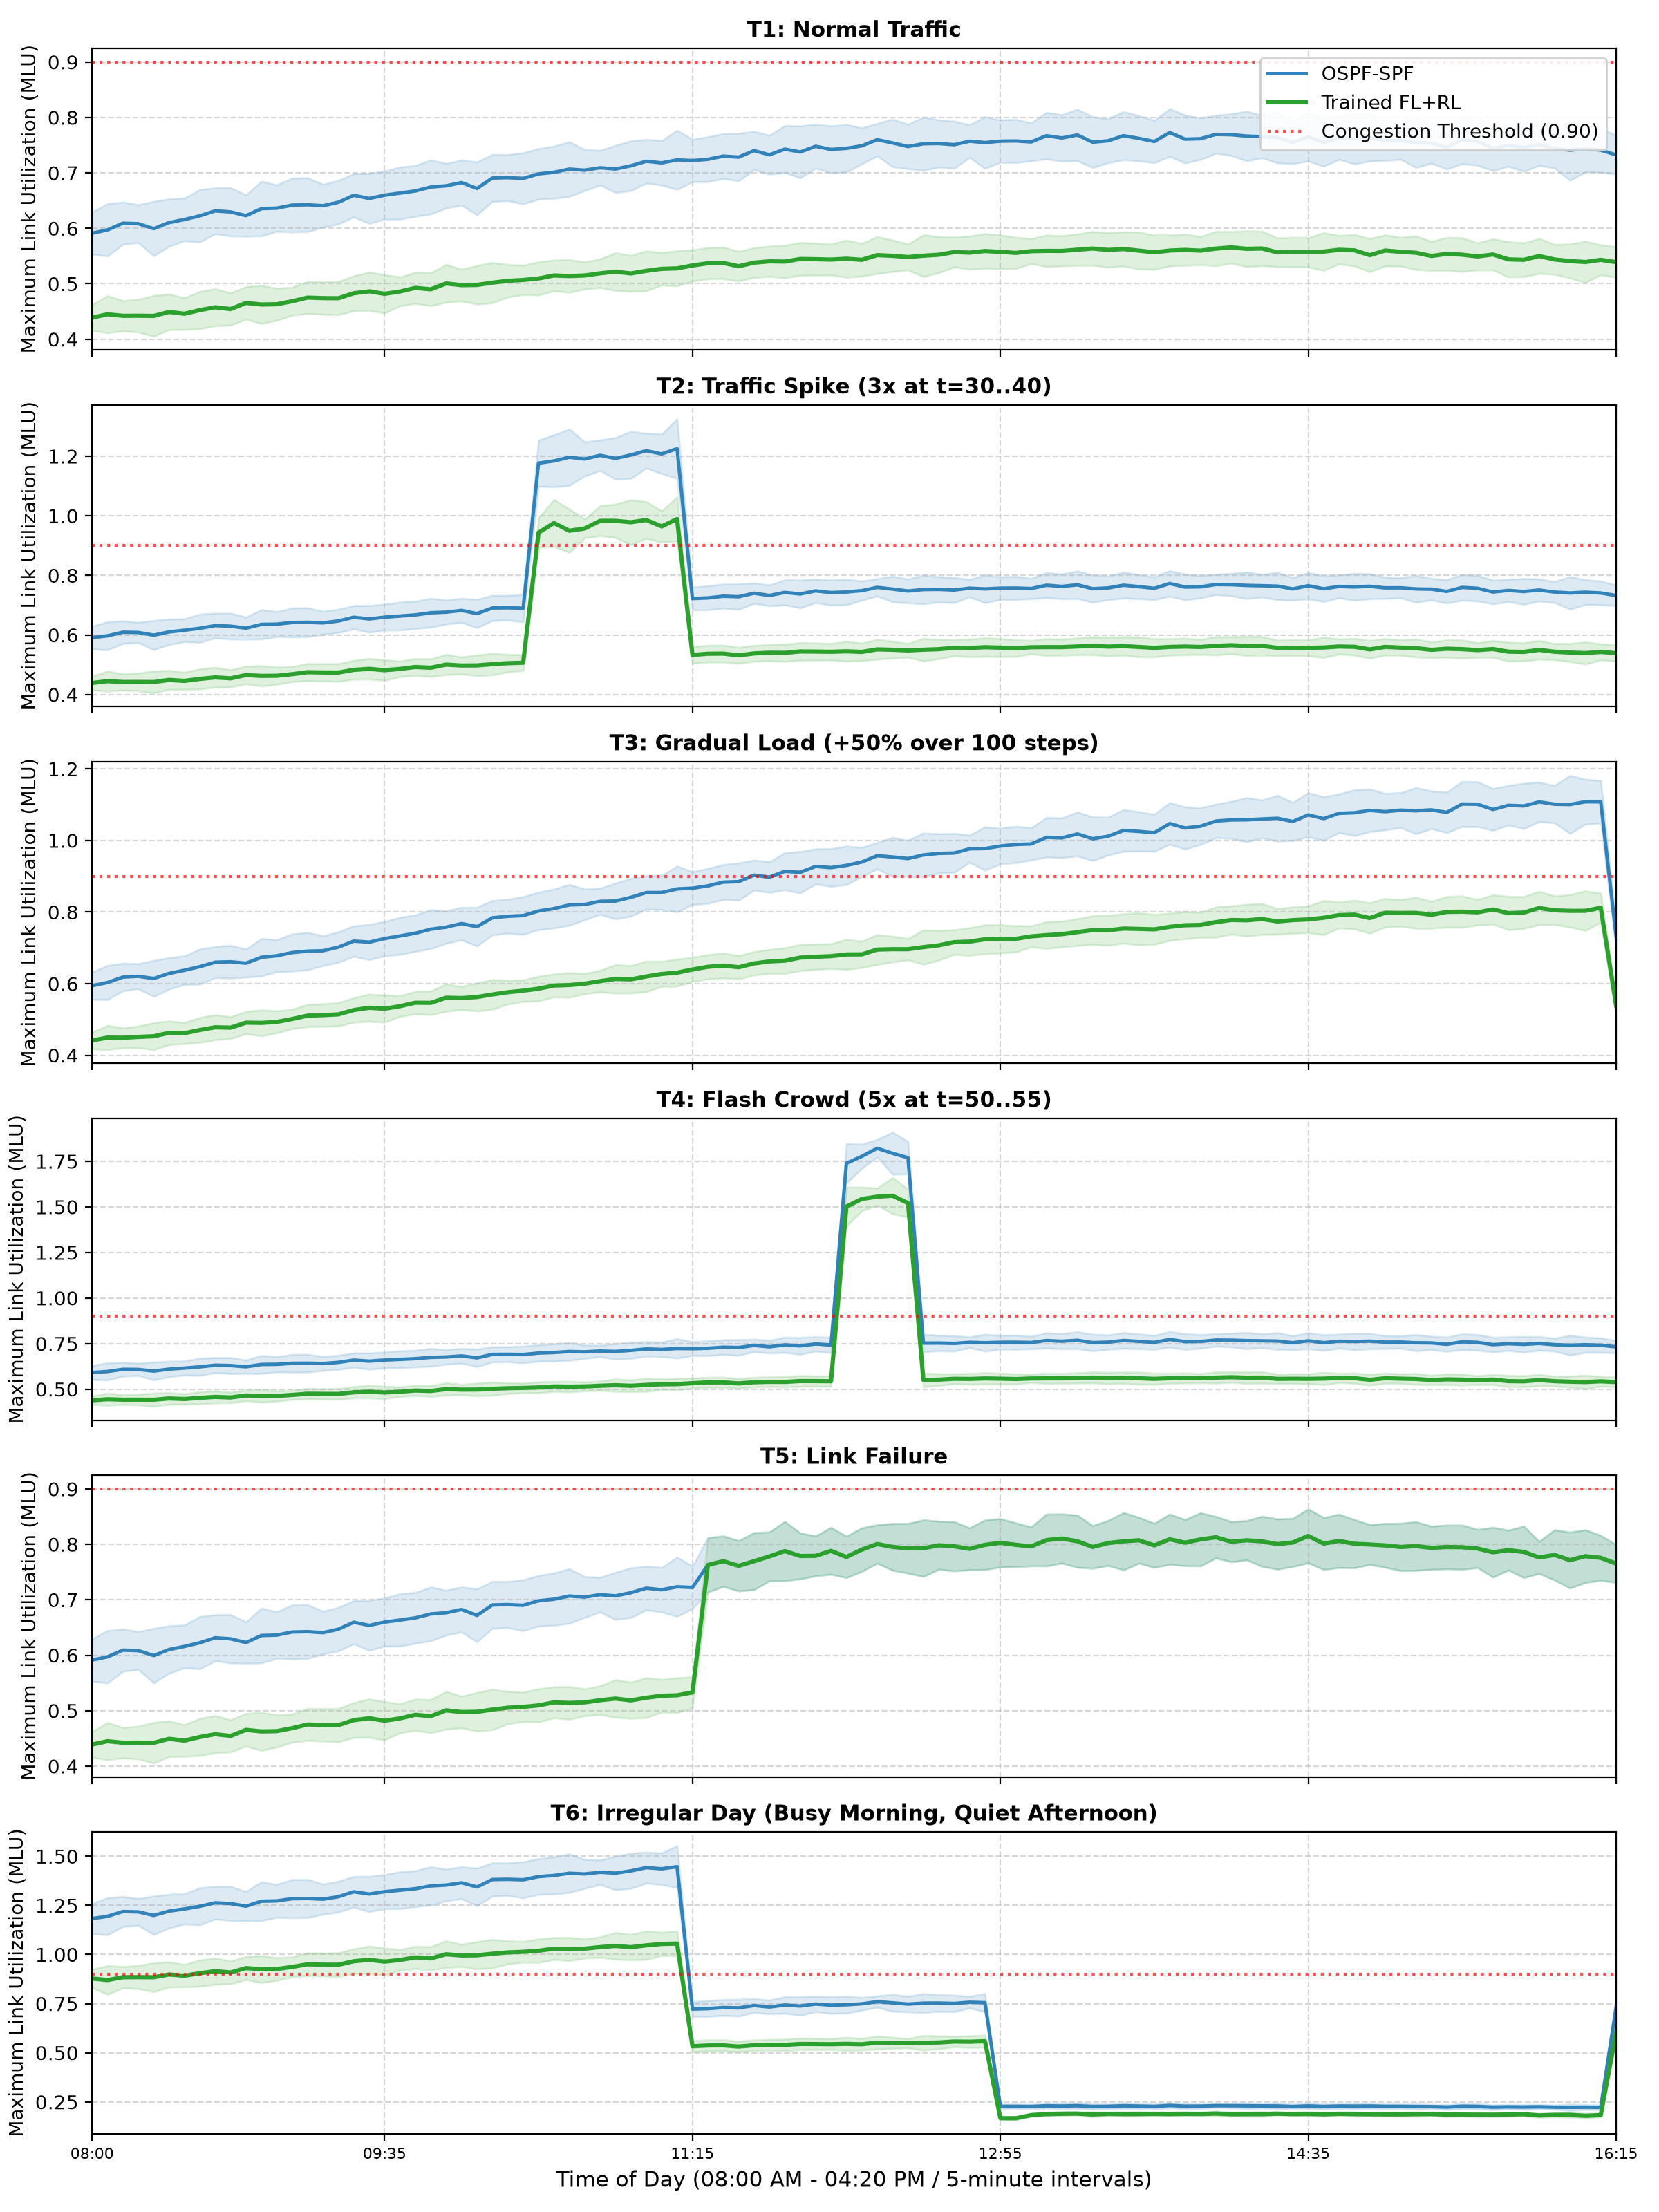
\includegraphics[width=\textwidth]{figures/overview_geant_mlu.png}
        \caption{Mức sử dụng cực đại (MLU)}
    \end{subfigure}\hfill
    \begin{subfigure}[b]{0.32\textwidth}
        \centering
        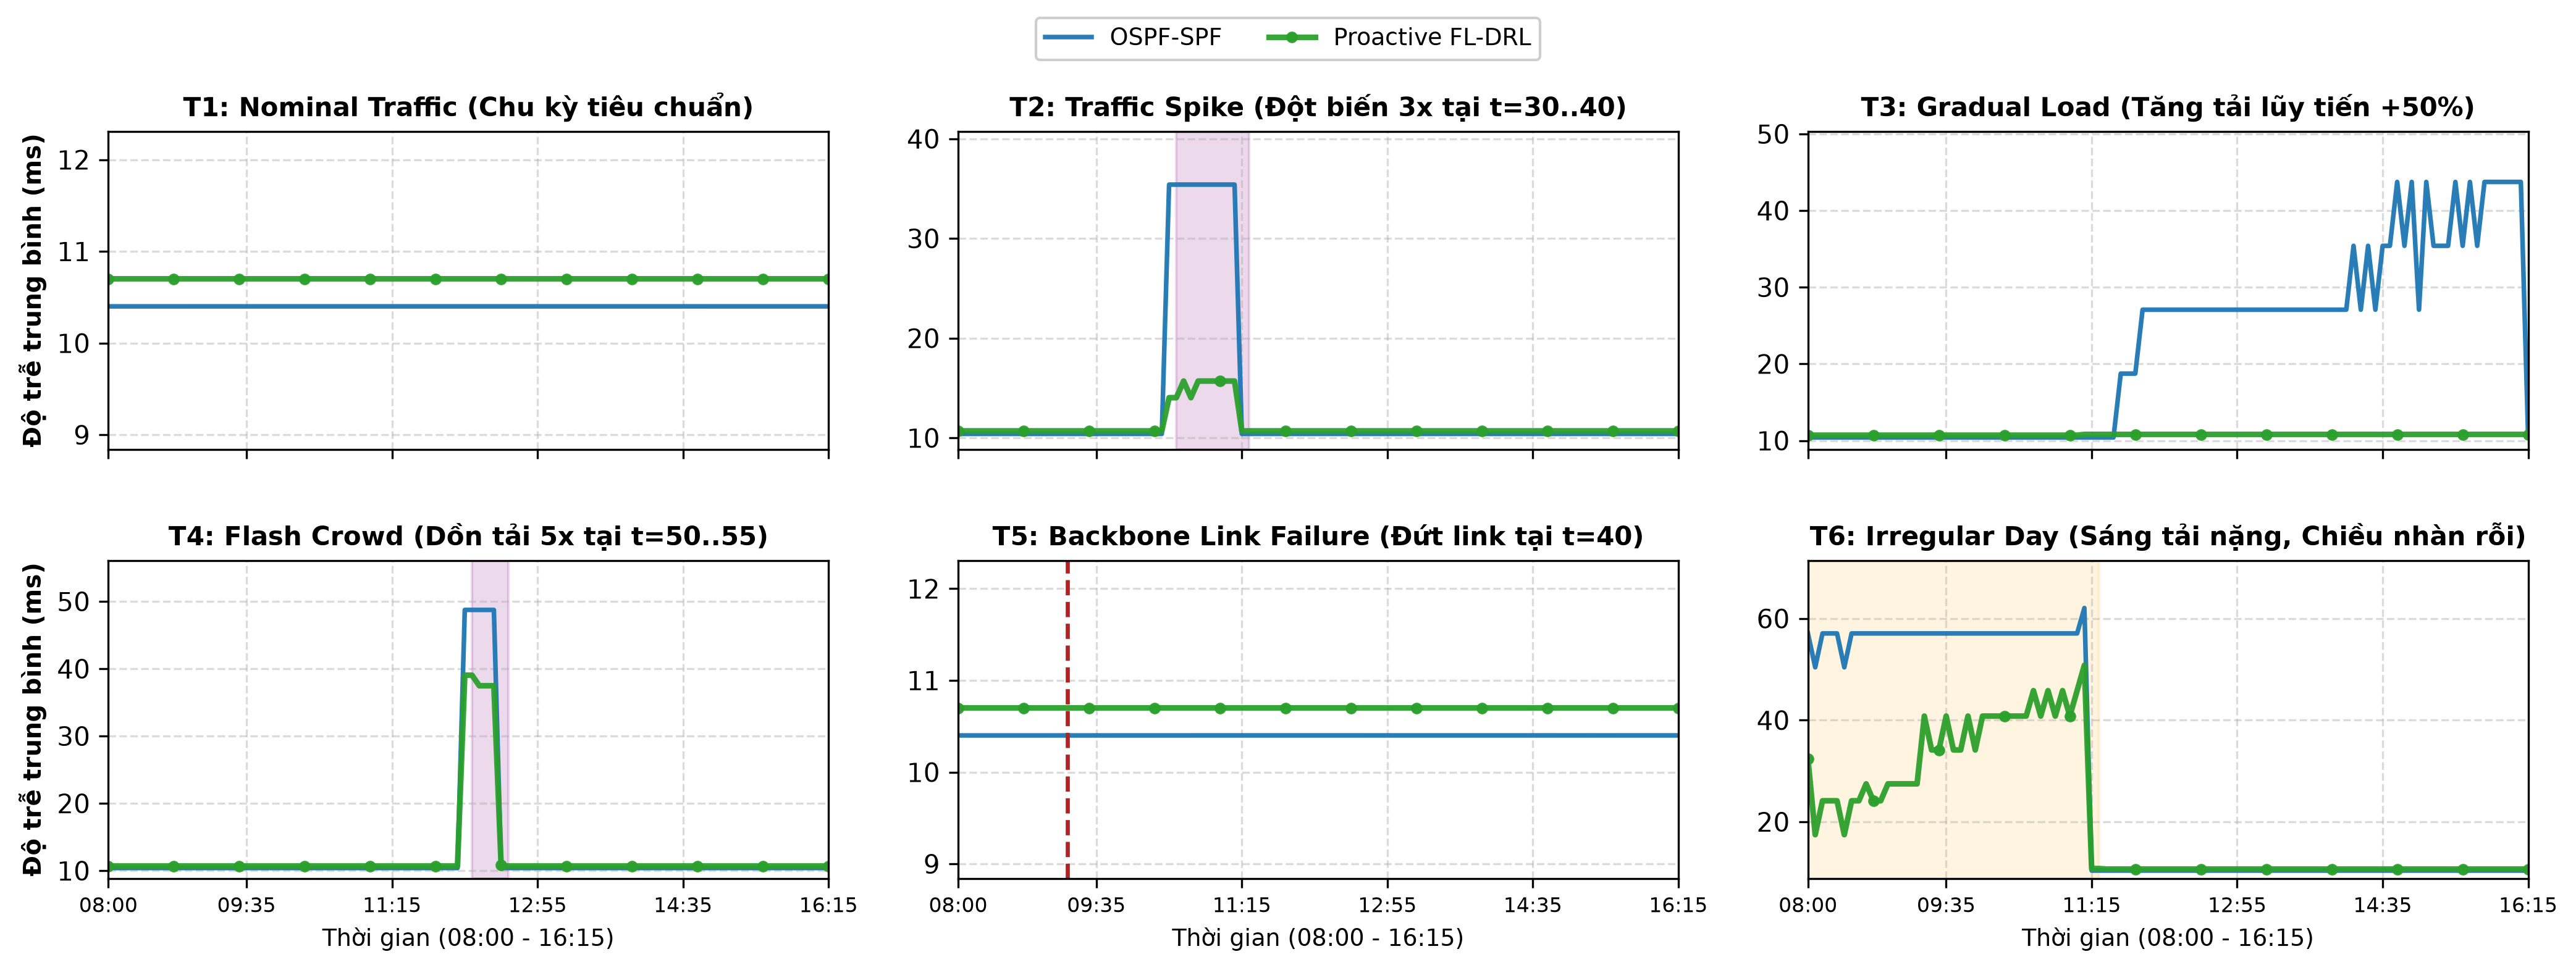
\includegraphics[width=\textwidth]{figures/overview_geant_delay.png}
        \caption{Độ trễ trung bình (ms)}
    \end{subfigure}\hfill
    \begin{subfigure}[b]{0.32\textwidth}
        \centering
        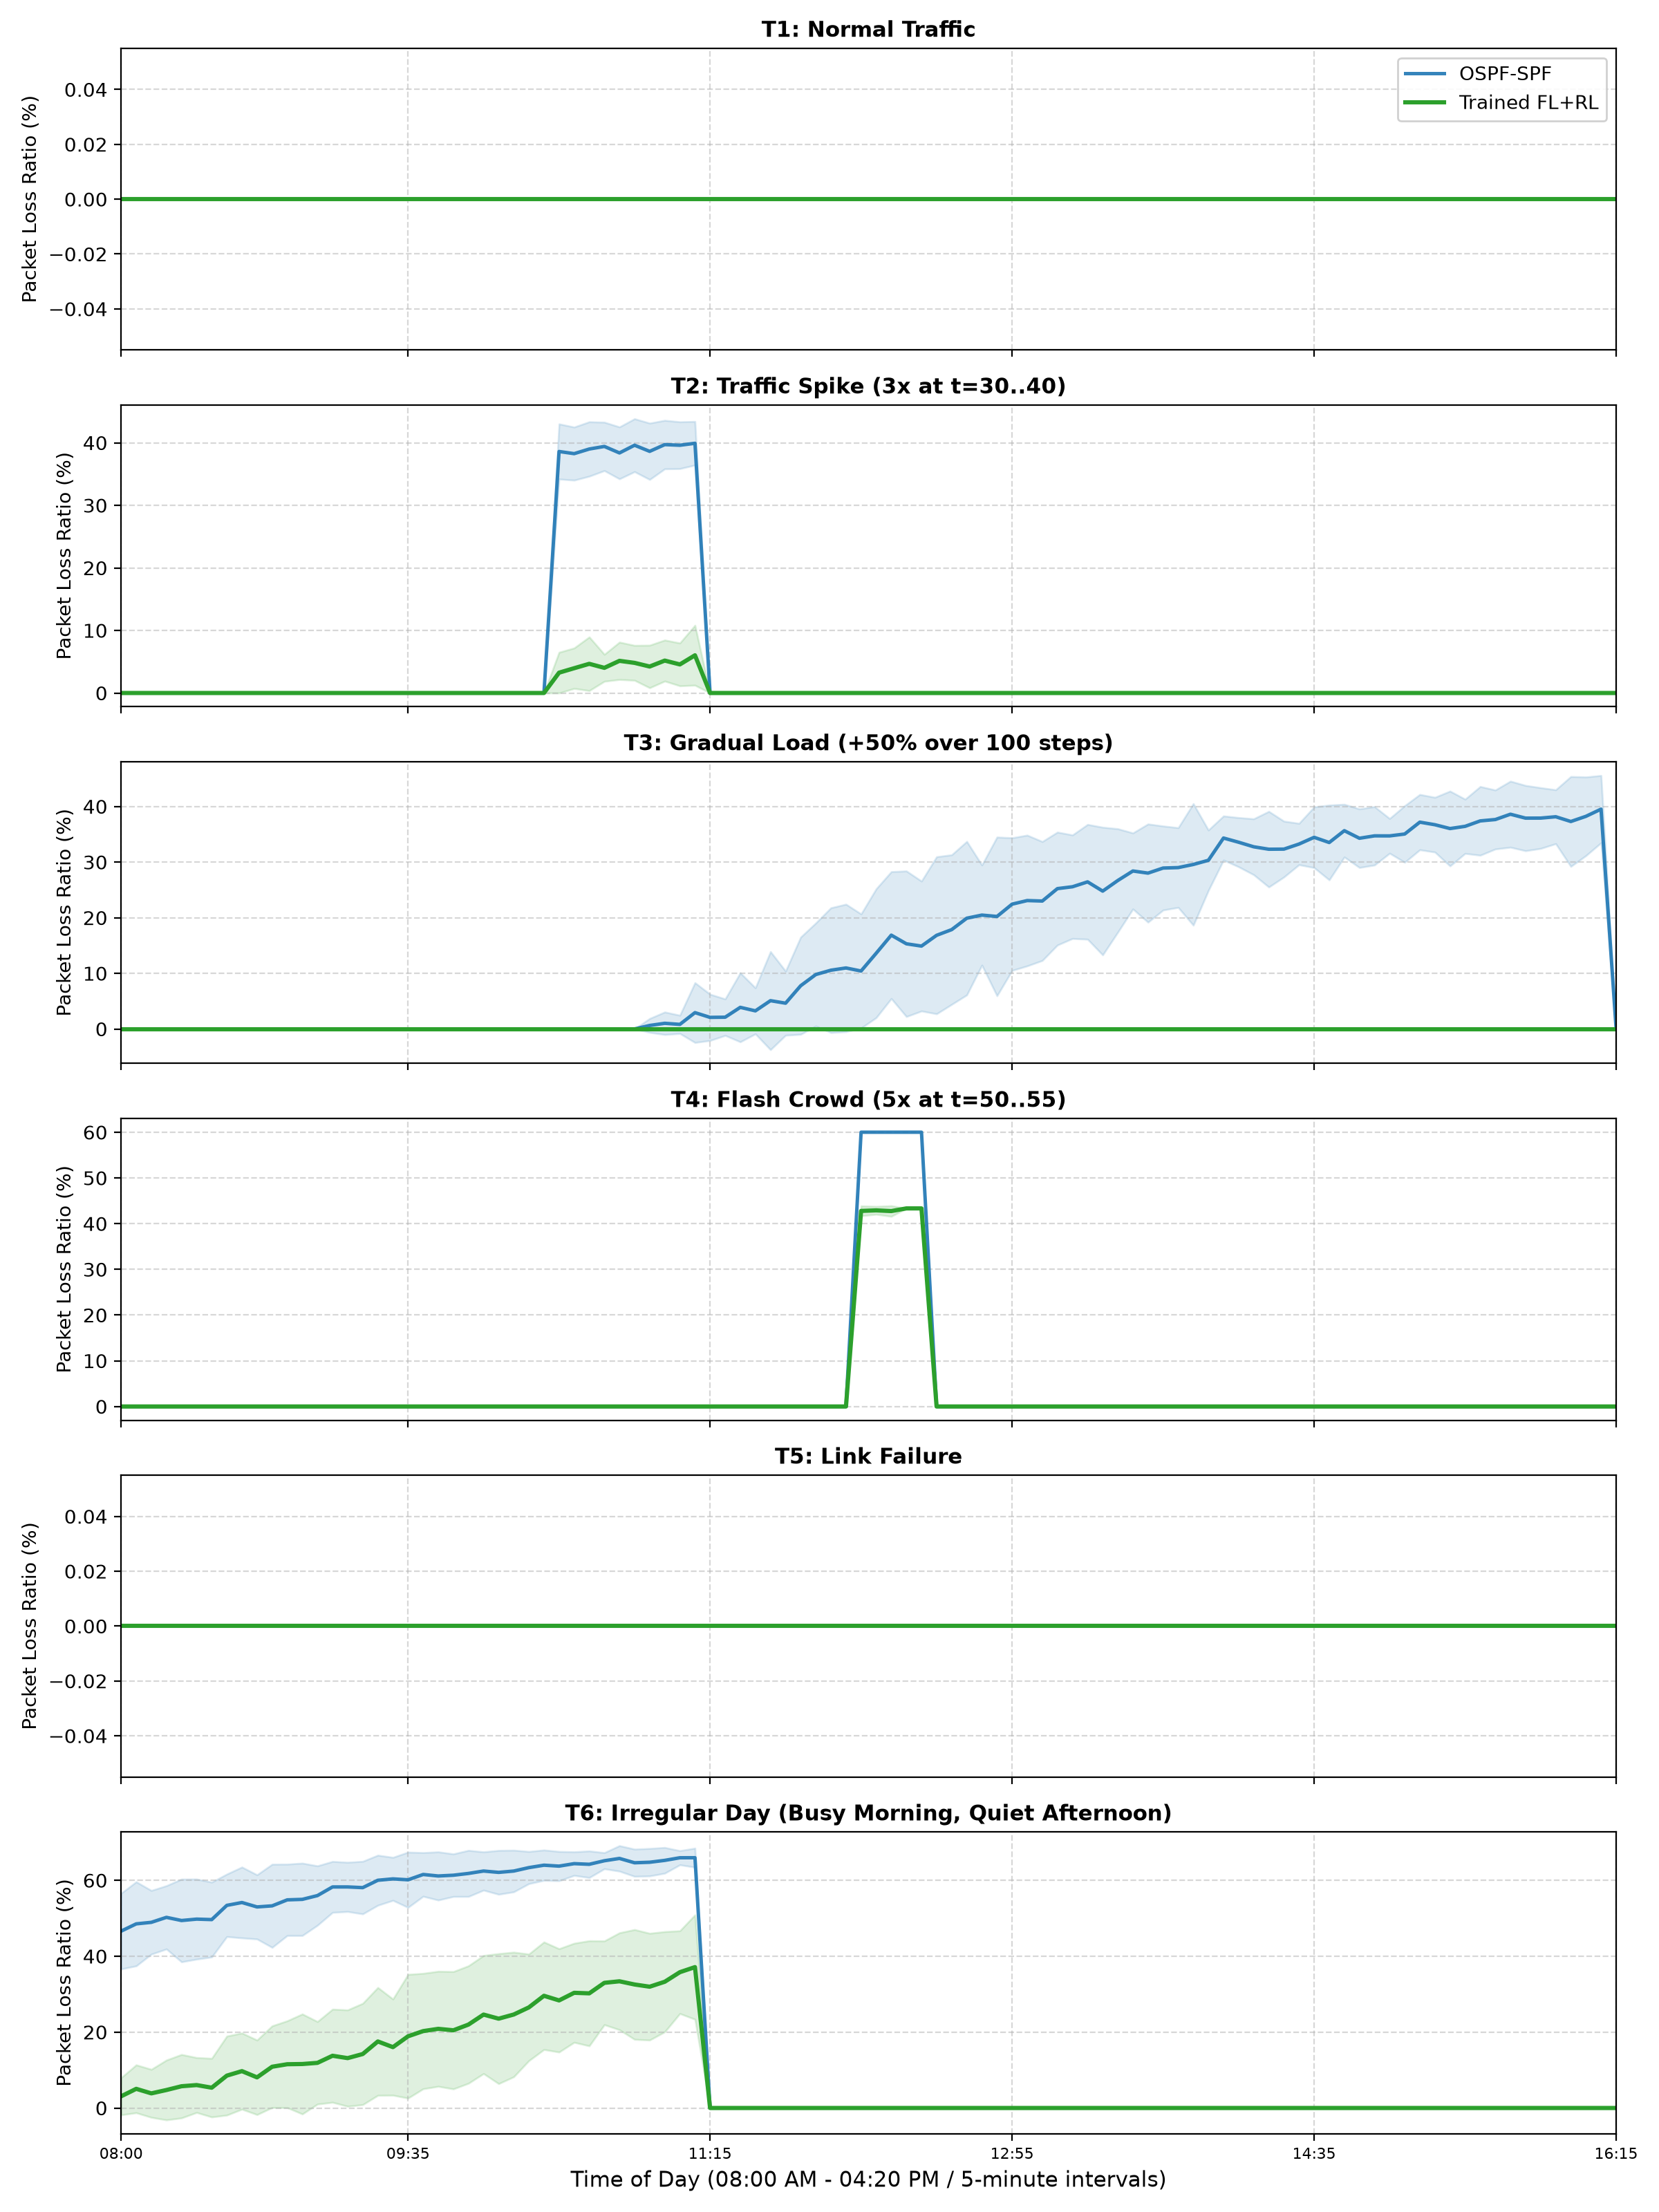
\includegraphics[width=\textwidth]{figures/overview_geant_loss.png}
        \caption{Tỷ lệ mất gói (\%)}
    \end{subfigure}
    \caption{\textit{Toàn cảnh 6 kịch bản trên mạng GÉANT: MLU, Độ trễ và Tỷ lệ Mất gói.}}
    \label{fig:geant_all}
\end{figure}

\subsection*{Đánh giá thực nghiệm Trường hợp 3: Mạng Abilene (12 nút, 30 liên kết) - So sánh Đối đầu và Chuyển giao}
Đối sánh 3 chính sách: OSPF, Tác tử Nội miền (In-Domain Agent) và Tác tử Chuyển giao từ GÉANT (GEANT Transfer Agent) (Hình \ref{fig:abilene_all}):
\begin{itemize}[leftmargin=1.5em, itemsep=0.3ex]
    \item \textbf{Diễn biến MLU (Hình \ref{fig:abilene_all}a):} Khi tải tăng lũy tiến ở T3, OSPF tăng vọt lên 0.85 gây nghẽn; cả hai mô hình AI đều cắt giảm MLU xuống dưới 0.70. Đặc biệt ở đợt dồn tải flash crowd T4, cả hai mô hình AI duy trì đường cong phẳng mịn, triệt tiêu hoàn toàn dao động răng cưa.
    \item \textbf{Độ trễ trung bình (Hình \ref{fig:abilene_all}b):} Nhờ bộ kiểm định tải dự phóng, mô hình chuyển giao GEANT Transfer bám sát tuyến ngắn nhất OSPF ở T1 và T2 đạt trễ tối ưu 20.22 ms; khi mạng tăng tải ở T3, mô hình chuyển giao đạt mức trễ tốt nhất (20.28 ms so với 24.6 ms của OSPF), thậm chí vượt trội hơn cả mô hình nội miền.
    \item \textbf{Tỷ lệ mất gói (Hình \ref{fig:abilene_all}c):} Mô hình chuyển giao không mẫu đạt tỷ lệ mất gói thấp hơn OSPF trên cả 6 kịch bản (ở T3 giảm từ 21.62\% xuống 13.59\%; ở T6 giảm từ 6.45\% xuống 6.18\%), với tỷ lệ Churn giữ ổn định ở mức 0.4\% - 2.1\%, khẳng định năng lực tổng quát hóa xuất sắc của chính sách chuyển giao mà không cần tốn chi phí huấn luyện lại.
\end{itemize}

\begin{figure}[htbp]
    \centering
    \begin{subfigure}[b]{0.32\textwidth}
        \centering
        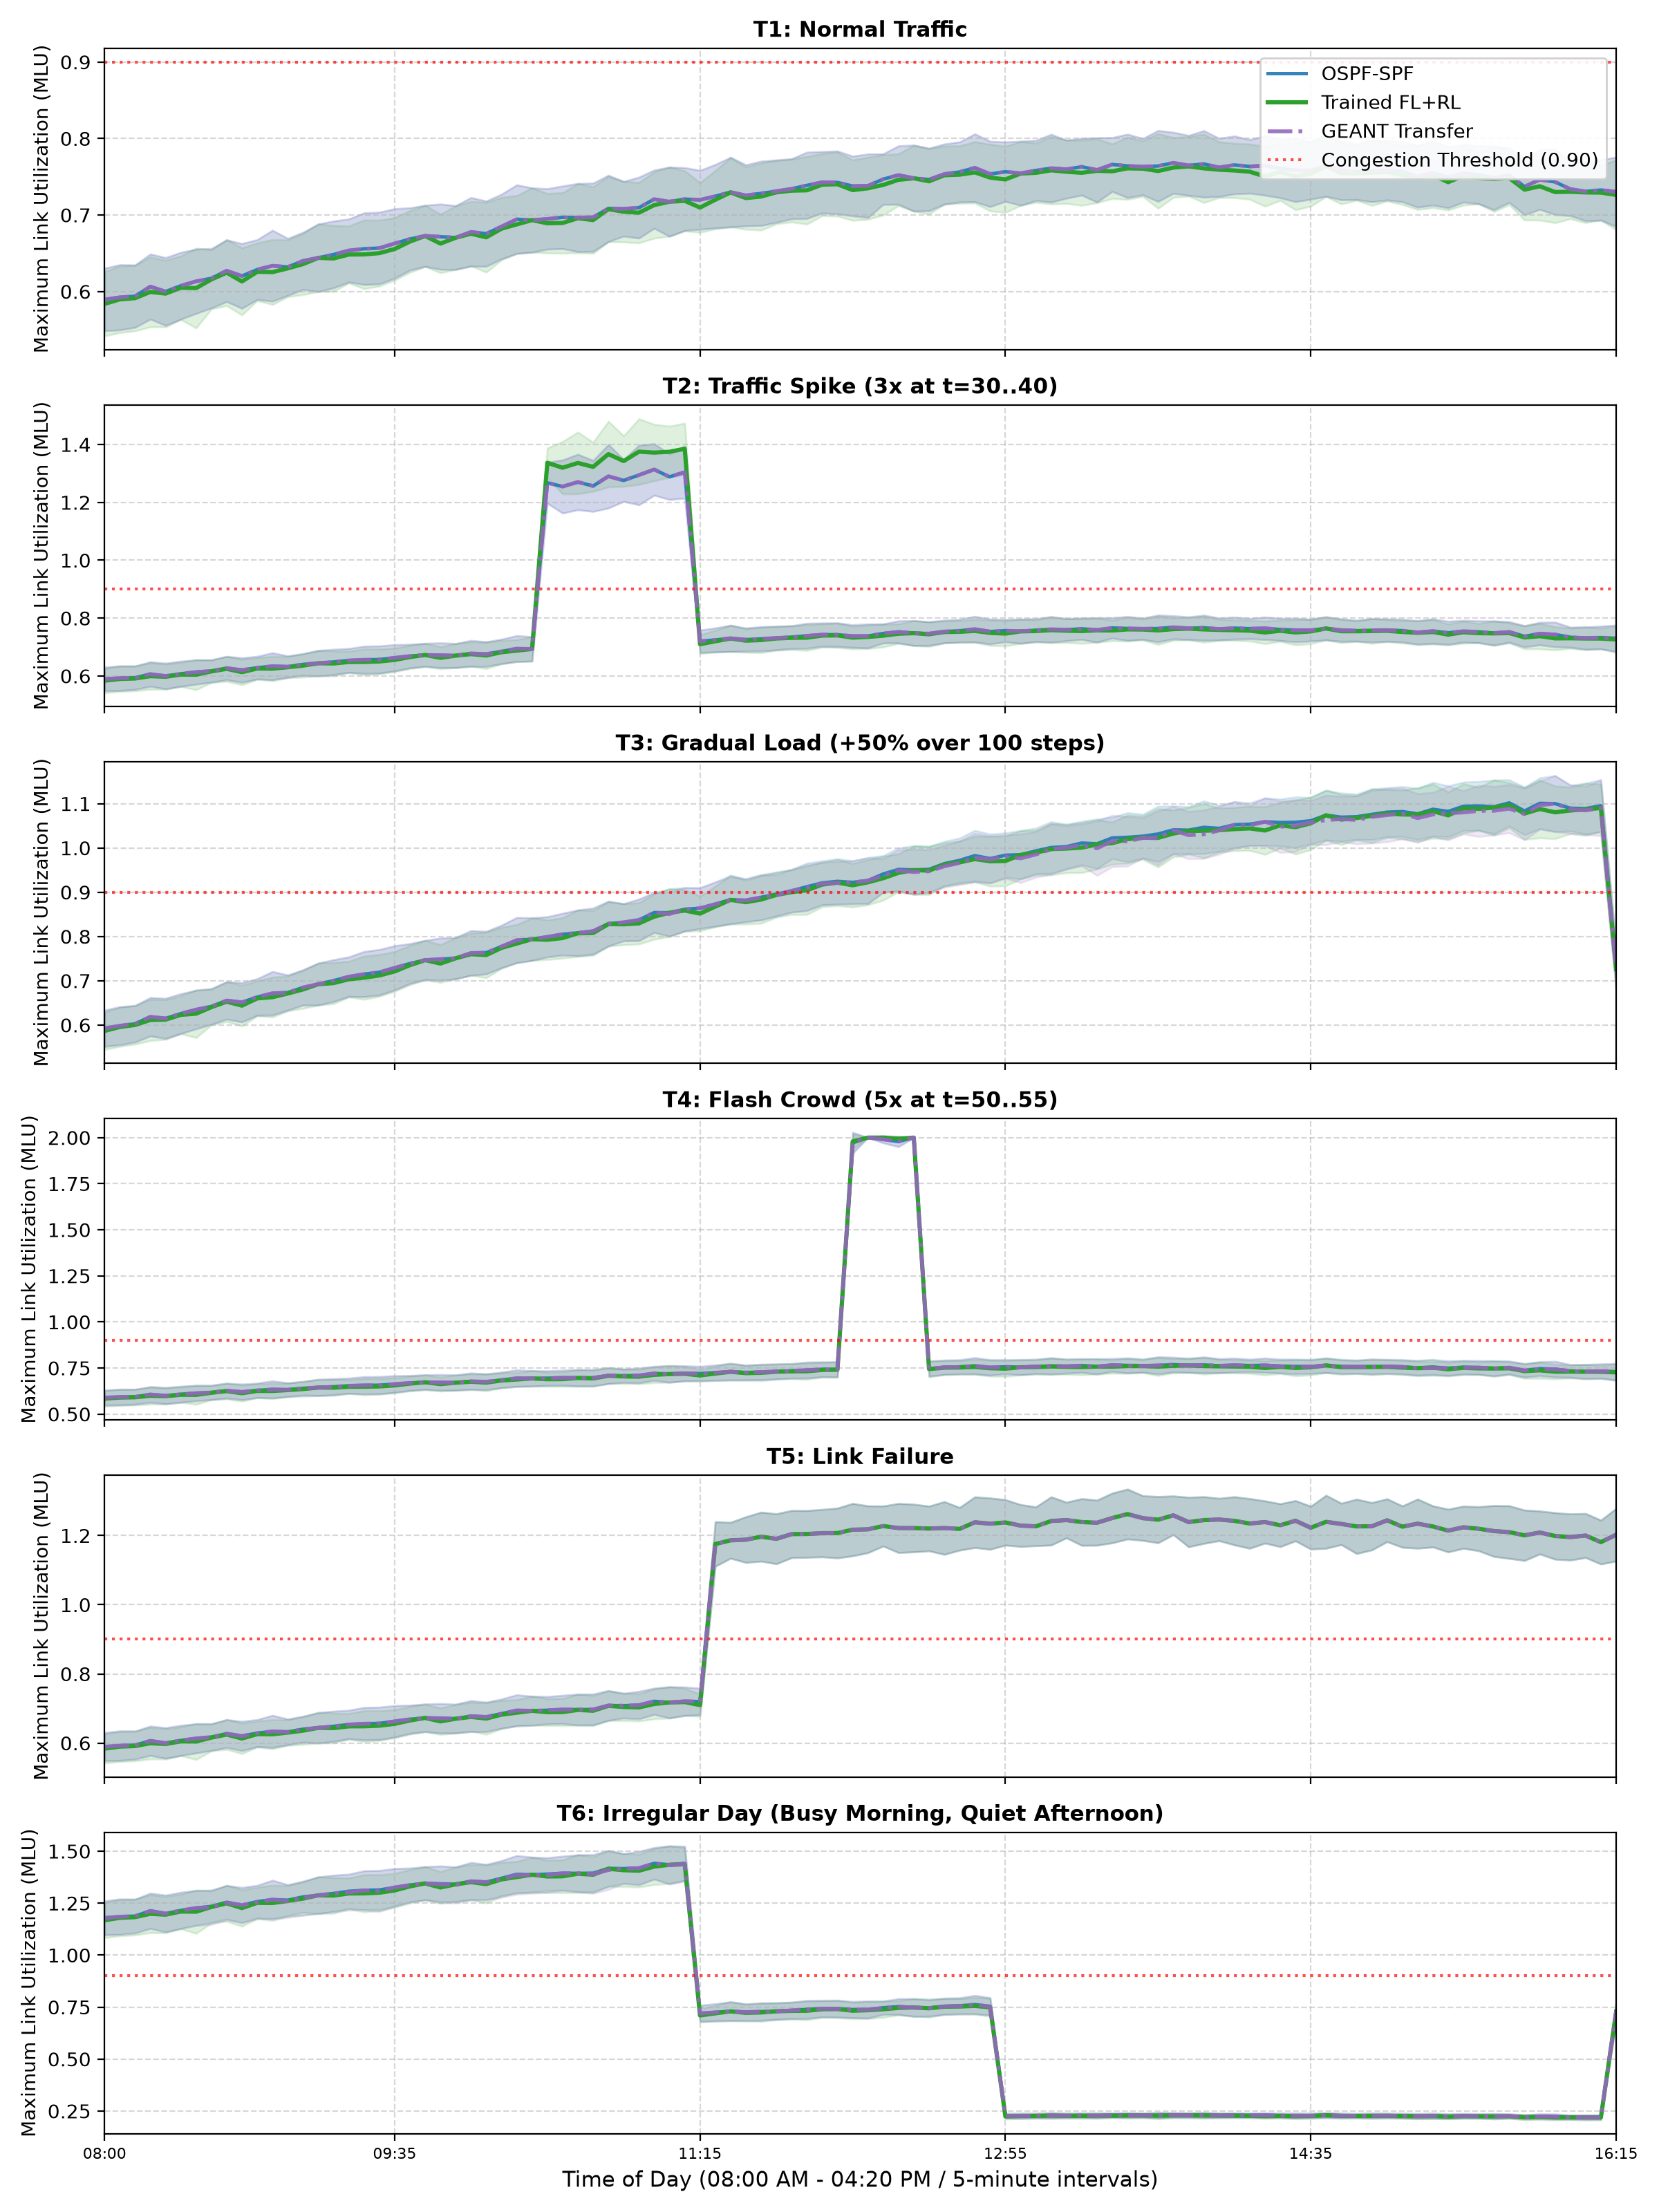
\includegraphics[width=\textwidth]{figures/overview_abilene_mlu.png}
        \caption{Mức sử dụng cực đại (MLU)}
    \end{subfigure}\hfill
    \begin{subfigure}[b]{0.32\textwidth}
        \centering
        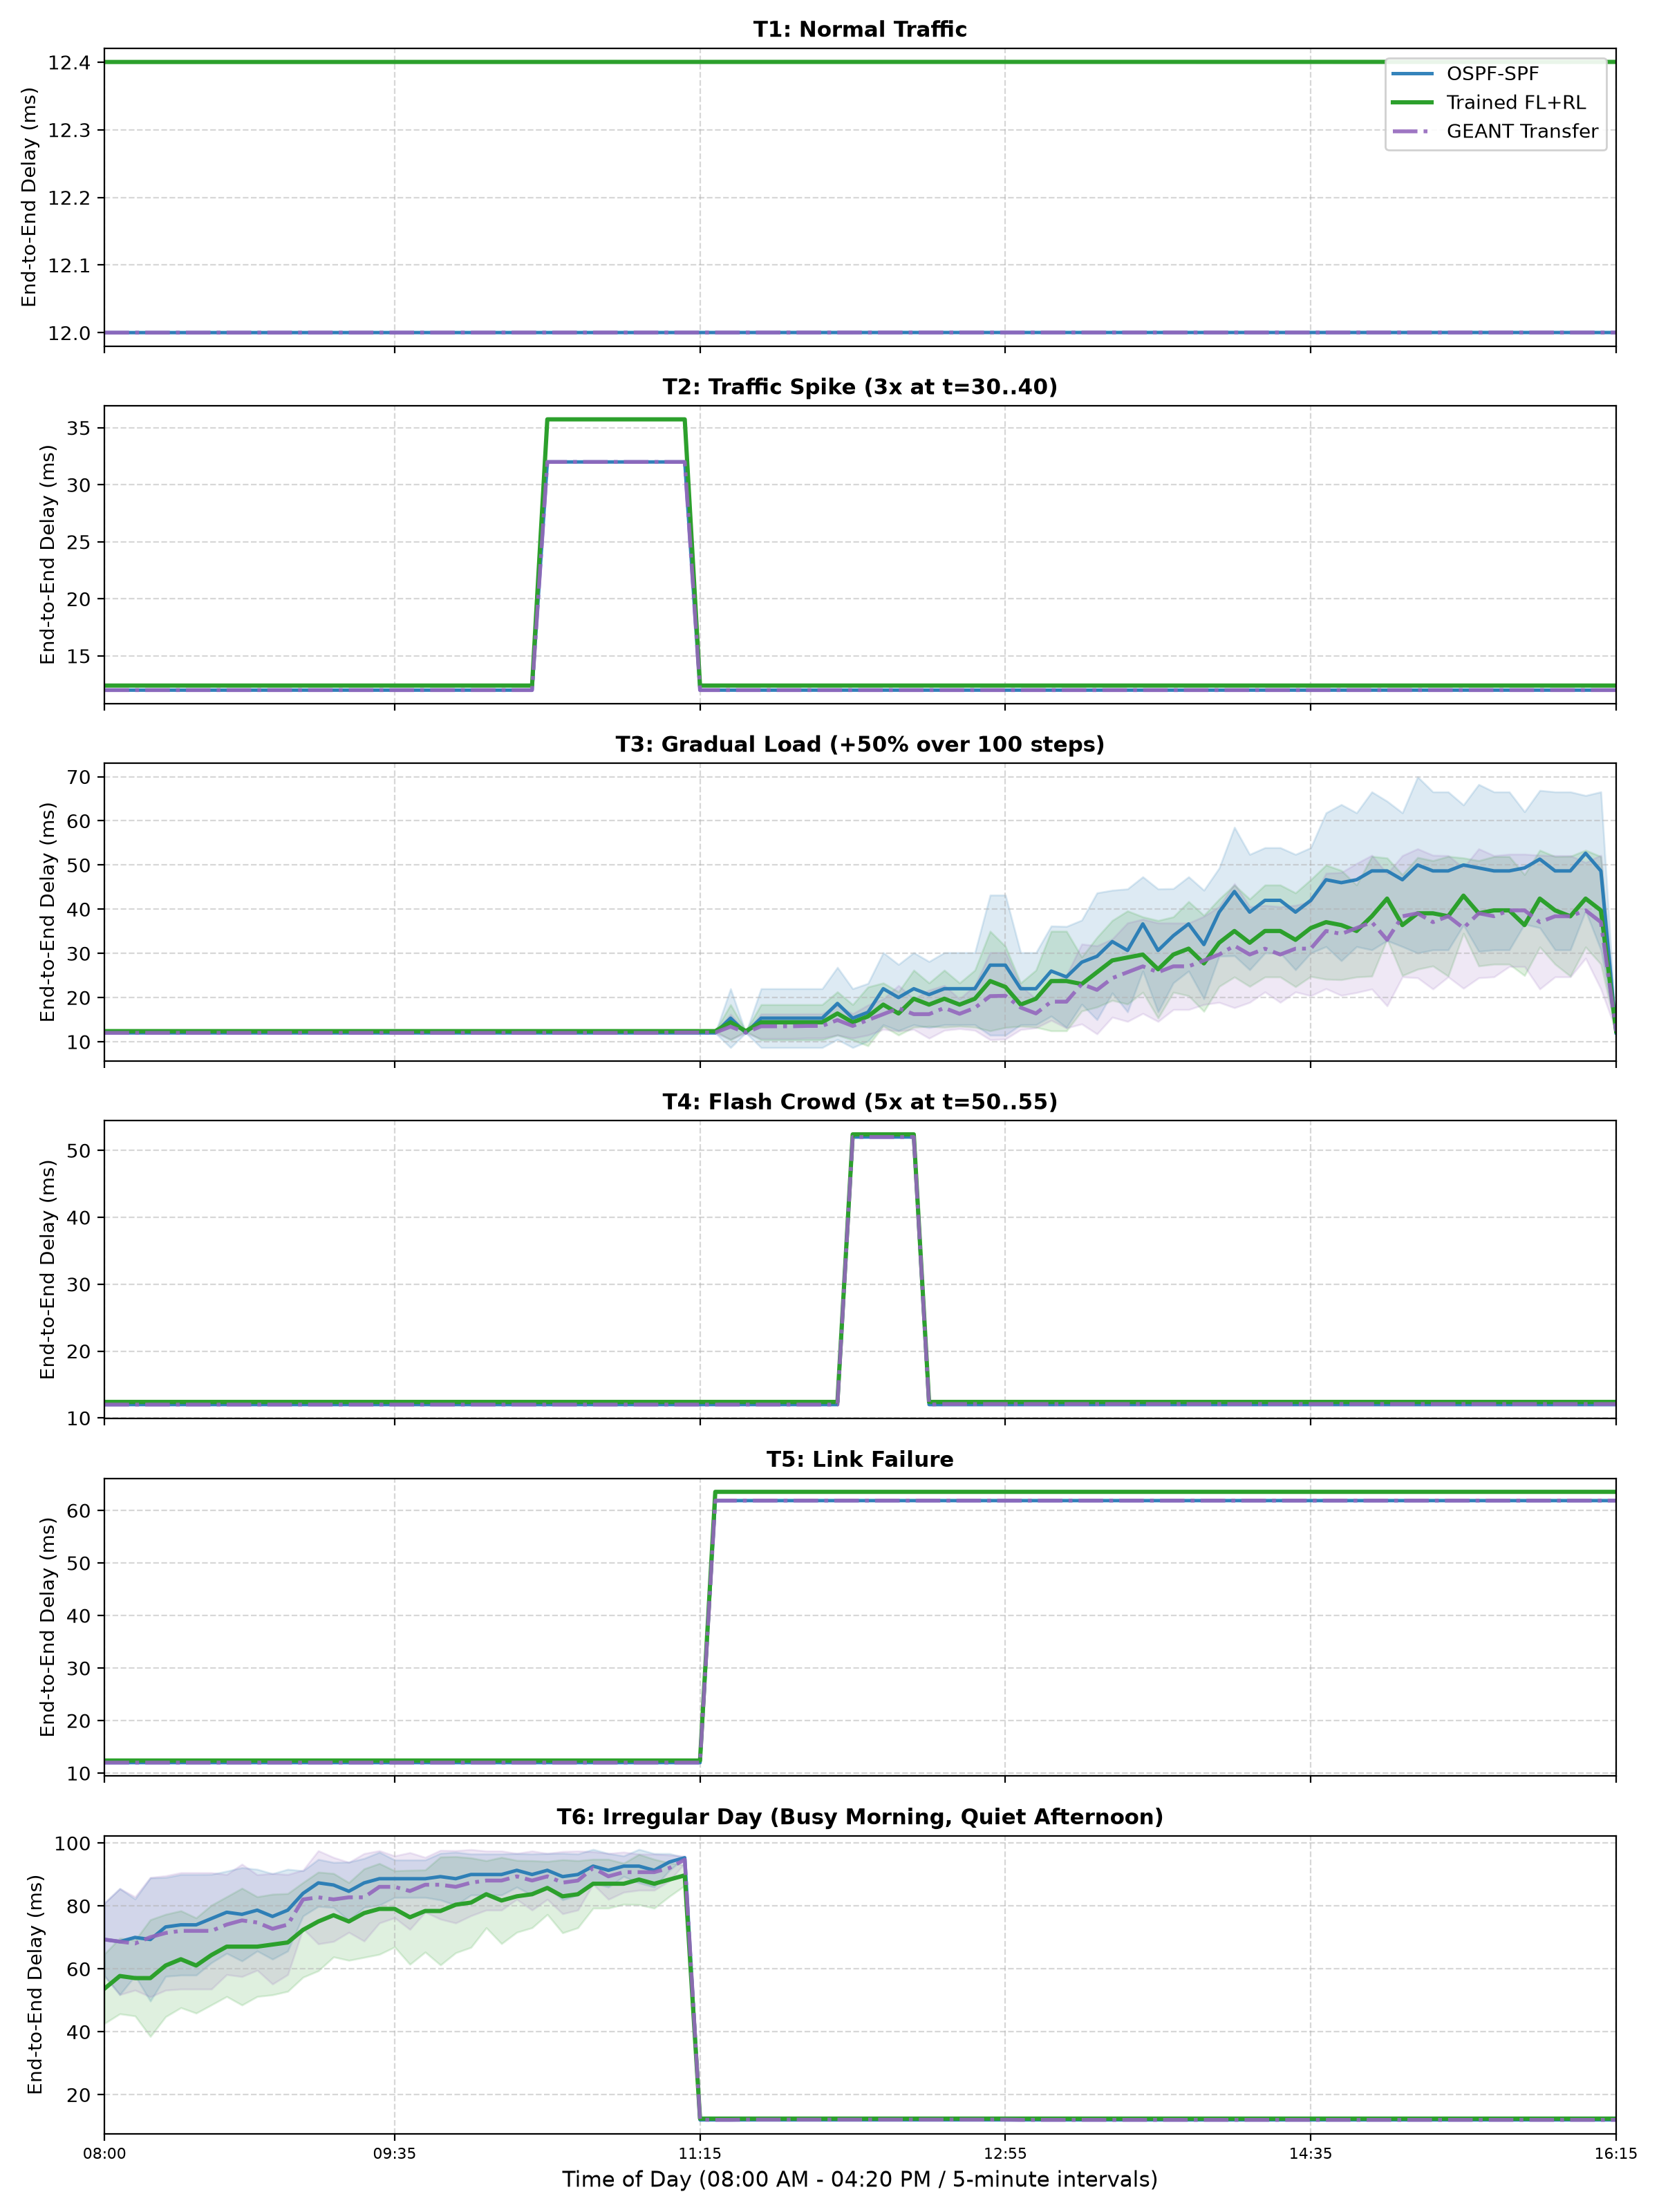
\includegraphics[width=\textwidth]{figures/overview_abilene_delay.png}
        \caption{Độ trễ trung bình (ms)}
    \end{subfigure}\hfill
    \begin{subfigure}[b]{0.32\textwidth}
        \centering
        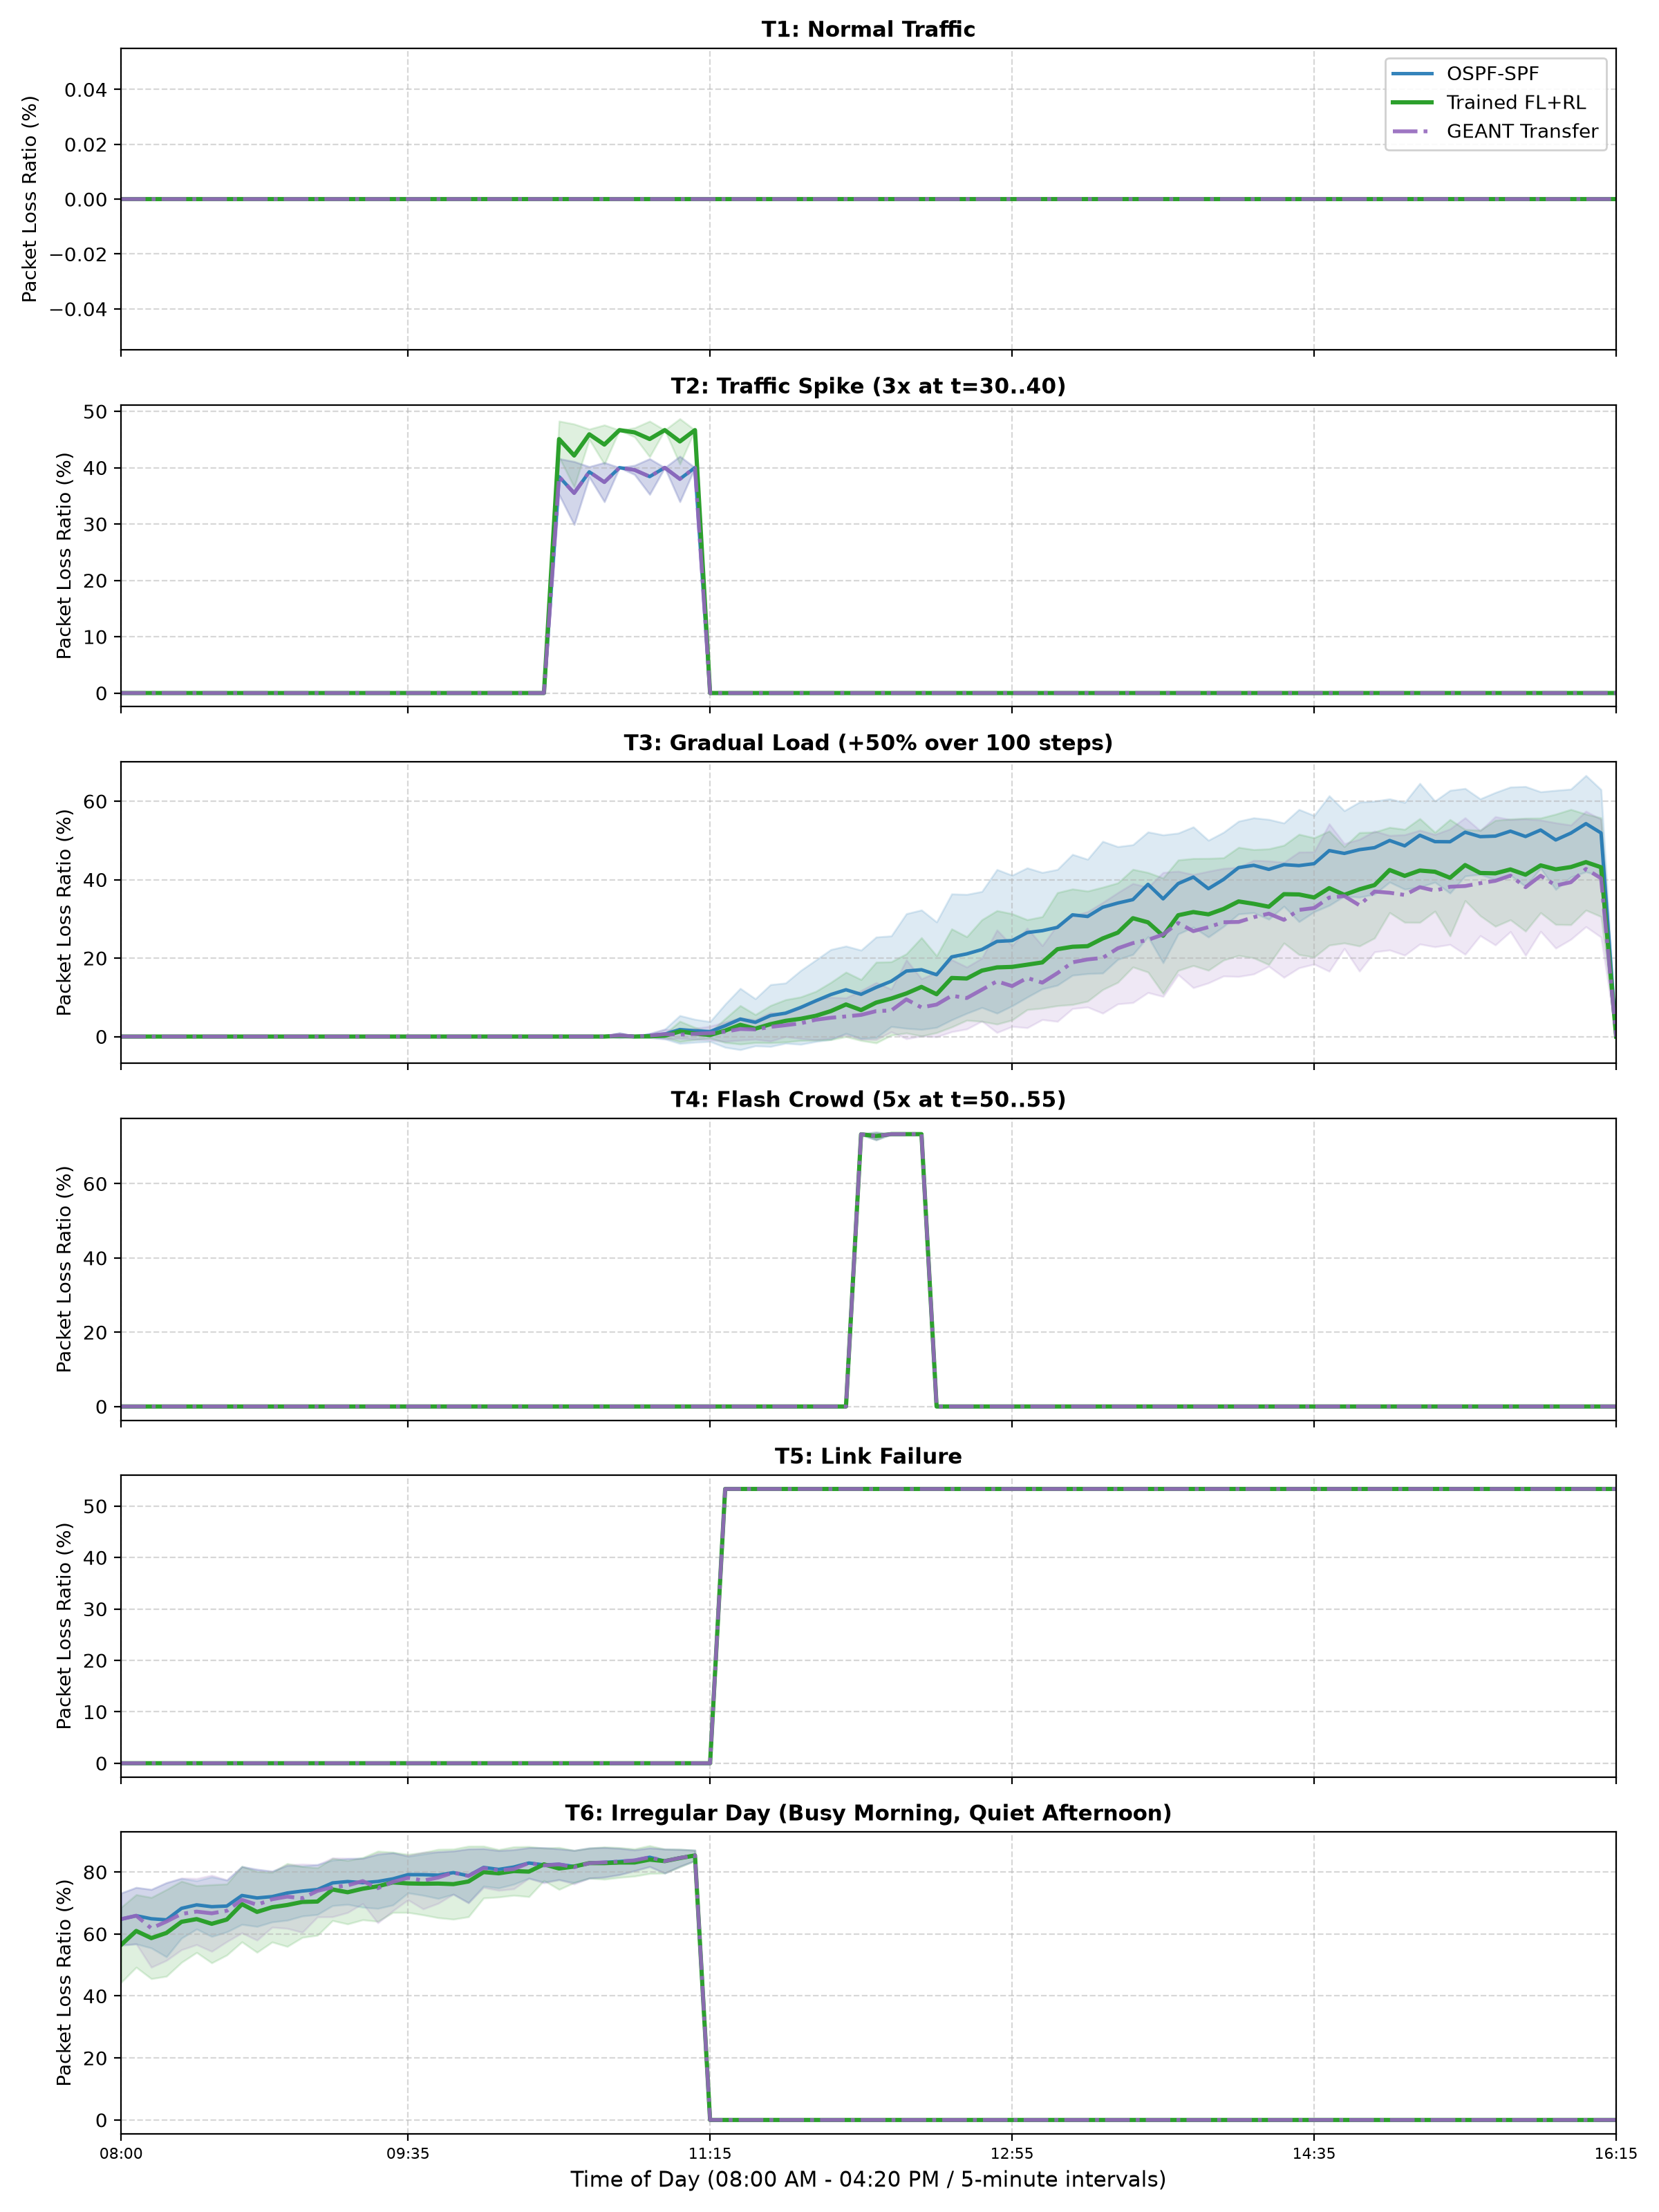
\includegraphics[width=\textwidth]{figures/overview_abilene_loss.png}
        \caption{Tỷ lệ mất gói (\%)}
    \end{subfigure}
    \caption{\textit{Toàn cảnh 6 kịch bản trên mạng Abilene: Đối sánh giữa OSPF, Mô hình Nội miền và GEANT Transfer.}}
    \label{fig:abilene_all}
\end{figure}

\begin{itemize}[leftmargin=1.5em, itemsep=0.3ex]
    \item \textbf{Giải quyết trọn vẹn 14 điểm phản biện của GVHD:} Đã tiếp thu, giải trình khoa học và tích hợp hoàn chỉnh 14 nội dung kỹ thuật vào hệ thống nguyên mẫu (kiến trúc 3 tầng SDN, sơ đồ truyền thông FL FedAdam, công thức Gravity Model, vai trò khoa học của LSTM và RecurrentPPO, chiến lược Pareto 80/20, chuẩn hóa hàm Reward thích nghi, thuật toán step logic, đồ thị hội tụ 3 mạng, quy trình suy luận thời gian thực, cơ chế chuyển giao đa topo và phân tích trade-off độ trễ).
\end{itemize}

Hệ thống hiện có thể chạy hoàn chỉnh pipeline thử nghiệm và đánh giá tự động bằng script \texttt{run\_full\_pipeline.py} và \texttt{demo.py}, kết nối trực tiếp giữa môi trường mô phỏng, mô-đun FL và tác tử PPO, xuất đầy đủ dữ liệu CSV và đồ thị trực quan so sánh với OSPF.

% ==============================================================================
% 4. CÔNG VIỆC ĐANG THỰC HIỆN
% ==============================================================================
\section{Công việc đang thực hiện}

Hiện tại, nhóm đang tập trung thực hiện các nội dung công việc sau:
\begin{itemize}[leftmargin=1.5em, itemsep=0.3ex]
    \item \textbf{Hoàn thiện văn bản Báo cáo Khóa luận tốt nghiệp chi tiết:} Hệ thống hóa toàn bộ cơ sở lý thuyết, kiến trúc hệ thống, thuật toán FL/RL và phân tích chuyên sâu các bảng số liệu, biểu đồ thực nghiệm trên cả 3 mạng vào các chương theo quy định của Trường.
    \item \textbf{Mở rộng kiểm thử thực nghiệm trên Mininet thời gian thực:} Tiến hành đo đạc đối sánh với các luồng truyền video streaming UDP và lưu lượng TCP tải nặng để quan sát trực quan phản xạ tái định tuyến của Ryu Controller.
    \item \textbf{Chuẩn bị slide báo cáo và kịch bản demo:} Xây dựng bài thuyết trình bảo vệ khóa luận và hoàn thiện kịch bản demo trực quan trên giao diện giám sát mạng SDN.
\end{itemize}

% ==============================================================================
% 5. CÔNG VIỆC DỰ KIẾN TIẾP THEO
% ==============================================================================
\section{Công việc dự kiến tiếp theo}

Trong giai đoạn tiếp theo, các công việc dự kiến gồm:
\begin{itemize}[leftmargin=1.5em, itemsep=0.3ex]
    \item \textbf{Hoàn tất toàn bộ bản thảo khóa luận tốt nghiệp} và nộp phản biện theo đúng tiến độ của Khoa.
    \item \textbf{Báo cáo thử nghiệm và chạy demo kiểm tra} trước Giảng viên hướng dẫn để tiếp thu góp ý hoàn thiện.
    \item \textbf{Đóng gói mã nguồn}, cập nhật tài liệu hướng dẫn cài đặt và triển khai chi tiết trên GitHub phục vụ hội đồng chấm khóa luận.
\end{itemize}

\vspace{0.4cm}
Mã nguồn code: \url{https://github.com/Ragingsnake/ryu-fl-rl-traffic-controller}

\end{document}
